\documentclass[a4paper,12pt]{article}
\RequirePackage{kvoptions-patch}
\RequirePackage{ifthen}
\usepackage[english]{babel}
\usepackage[utf8]{inputenc}
\usepackage{url}
\usepackage{graphicx}
\graphicspath{ {imgs/} }
\usepackage{floatrow}
\usepackage{amsfonts}
\usepackage{amssymb}
\usepackage{algorithm2e}
\usepackage{newclude}
\usepackage{amsmath}
\usepackage{hyperref}
\usepackage{cleveref}
\usepackage{multirow}
\usepackage[toc,page]{appendix}

\usepackage{longtable}
\usepackage[acronym]{glossaries}
\usepackage{acro}

\usepackage{enumerate}% http://ctan.org/pkg/enumerate


%table
\usepackage{array}
\usepackage[a4paper]{geometry}
\usepackage{tabularx}
\usepackage{lipsum}
%\newcolumntype{M}[1]{>{\centering\arraybackslash}m{#1}}
%\newcolumntype{N}{@{}m{0pt}@{}}

% make paragraph start a new line instead of indent
\usepackage[parfill]{parskip}

% Glossary
%\makeglossaries
%\loadglsentries{acronyms}
%\newacronym{gcd}{GCD}{Greatest Common Divisor}

%%% to be done command
% set a to be done
\usepackage[textwidth=1.6cm]{todonotes}
\usepackage{xpatch}

\def\resetnamelevel#1{%
    \ifnum#1<1\let\thischaptername\relax\fi
    \ifnum#1<2\let\thissectionname\relax\fi
    \ifnum#1<3\let\thissubsectionname\relax\fi
    \ifnum#1<4\let\thissubsubsectionname\relax\fi
}\resetnamelevel{0}

\def\chaptername#1{\resetnamelevel{0}\def\thischaptername{#1}}
\def\sectionname#1{\resetnamelevel{1}\def\thissectionname{#1}}
\def\subsectionname#1{\resetnamelevel{2}\def\thissubsectionname{#1}}
\def\subsubsectionname#1{\resetnamelevel{3}\def\thissubsubsectionname{#1}}

\let\Chaptermark\chaptermark
\let\Sectionmark\sectionmark
\let\Subsectionmark\subsectionmark
\let\Subsubsectionmark\subsubsectionmark
\def\chaptermark#1{\chaptername{#1}\Chaptermark{#1}}
\def\sectionmark#1{\sectionname{#1}\Sectionmark{#1}}
\def\subsectionmark#1{\subsectionname{#1}\Subsectionmark{#1}}
\def\subsubsectionmark#1{\subsubsectionname{#1}\Subsubsectionmark{#1}}

\makeatletter
\newcommand\treeloc{%
    \ifx\thischaptername\relax%
        ??\@latex@warning{\textbackslash treeloc called outside of structure}
    \else
        \thischaptername%
        \ifx\thissectionname\relax%
        \else
            \ /\ \thissectionname%
            \ifx\thissubsectionname\relax%
            \else
                \ /\ \thissubsectionname%
                \ifx\thissubsubsectionname\relax%
                \else
                    \ /\ \thissubsubsectionname%
                \fi
            \fi
        \fi
    \fi
    }
\makeatother

\newcommand\tbd{%
    \todo[caption={TBD: \expandafter\treeloc}]{TBD}
}


%add an extra level of sections
\usepackage{titlesec}

\setcounter{secnumdepth}{4}

\titleformat{\paragraph}
{\normalfont\normalsize\bfseries}{\theparagraph}{1em}{}
\titlespacing*{\paragraph}
{0pt}{3.25ex plus 1ex minus .2ex}{1.5ex plus .2ex}

\usepackage[
title={3D Pose Estimation of Vehicles from Monocular Videos using Deep Learning},
author={Qing Cheng},
type=master,
institute=ipvs, % or other institute names - or just a plain string using {Demo\\Demo...}
course={INFOTECH},
examiner={Ph.D.\ Daniel Hennes},
supervisor={Ph.D.\ Hung Ngo, Jie Zhong},
startdate={January 1, 2018},
enddate={July 3, 2018},
language=english
]{scientific-thesis-cover}

\newacronym{DDT}{DDT}{Dynamic Driving Task}
\newacronym{OEDR}{OEDR}{Object and Event Detection and Response}
\newacronym{ODD}{ODD}{Operational Design Domain}
\newacronym{ADS}{ADS}{Active Safety Systems}
\newacronym{DARPA}{DARPA}{The Defense Advanced Research Projects Agency}
\newacronym{DL}{DL}{Deep Learning}
\newacronym{SVM}{SVM}{Support Vector Machine}
\newacronym{CNN}{CNN}{Convolutional Neural Network}
\newacronym{ILSVRC}{ILSVRC}{Large Scale Visual Recognition Challenge}
%\newacronym{}{}{}
%\newacronym{}{}{}
%\newacronym{}{}{}
%\newacronym{}{}{}
%\newacronym{}{}{}
%\newacronym{}{}{}
%\newacronym{}{}{}
\makeindex


%Begining of the document
\begin{document}
\Coverpage

%\begin{titlepage}
	\centering
%	\includegraphics[width=0.15\textwidth]{example-image-1x1}\par\vspace{1cm}
	{\scshape\LARGE Universität Stuttgart \par}
	\vspace{1cm}
	{\scshape\Large Master Thesis\par}
	\vspace{1.5cm}
	{\Large\bfseries 3D Pose Estimation of Vehicles from Monocular Videos using Deep Learning\par}
	\vspace{2cm}
	{\Large\itshape Qing Cheng\par}
	\vfill
	\
	Course of Study: Information Technology\par
	Examiner:         Ph.D. Daniel Hennes\par
	Supervisors:	Dr. Hung Ngo, Jie Zhong\par
	
	
	Commenced:    January 1, 2018\par
	Completed:        July 3, 2018\par
	
	\vfill
	
	% Bottom of the page
	{\large \par}
\end{titlepage}


\section*{Abstract}
In this thesis, we present a novel approach, Deep3DP, to perform 3D pose estimation of vehicles from monocular videos intended for autonomous driving scenarios. A robust deep neural network is applied to simultaneously perform 3D dimension proximity estimation, 2D part localization, and 2D part visibility prediction. In the inference phase, two of the learned features are fed to a pose estimation algorithm to estimate the 3D location, 3D orientation, and 3D dimensions of the vehicles with the help of a original 3D vehicle model dataset. Our approach can perform these six tasks simultaneously in real time and handle highly occluded or truncated vehicles. The experiment results show that our approach achieves state-of-the-art performance on six tasks and outperforms most of the monocular methods on the challenging KITTI benchmark.

\textbf{Keywords:} 3D pose estimation, 3D vehicle detection, KITTI, vehicle part location, vehicle part visibility, deep learning, computer vision
\clearpage

\tableofcontents
\clearpage
\listoffigures
\clearpage
\listoftables
\clearpage

%abbrevation
%\newacronym{DDT}{DDT}{Dynamic Driving Task}
\newacronym{OEDR}{OEDR}{Object and Event Detection and Response}
\newacronym{ODD}{ODD}{Operational Design Domain}
\newacronym{ADS}{ADS}{Active Safety Systems}
\newacronym{DARPA}{DARPA}{The Defense Advanced Research Projects Agency}
\newacronym{DL}{DL}{Deep Learning}
\newacronym{SVM}{SVM}{Support Vector Machine}
\newacronym{CNN}{CNN}{Convolutional Neural Network}
\newacronym{ILSVRC}{ILSVRC}{Large Scale Visual Recognition Challenge}
%\newacronym{}{}{}
%\newacronym{}{}{}
%\newacronym{}{}{}
%\newacronym{}{}{}
%\newacronym{}{}{}
%\newacronym{}{}{}
%\newacronym{}{}{}
%\printacronyms[include-classes=abbrev,name=Abbreviations]
%\printglossary[type=\acronymtype]


\section{Introduction}
\subsection{Motivation}
The autonomous vehicle (AV) is the evolutionary direction of automobiles due to its promising reliability and efficiency, as well as the underlying commercial profits.  The very essential step for AVs is to gain a comprehensive perception of the driving environment. Object detection is one of the key challenges of perception. Thanks to the remarkable advancement of deep neural networks, great achievements have been made on 2D object detection, while 3D object detection is still underdeveloped. For example, according to the  KITTI Object Detection Benchmark\cite{Geiger2012CVPR}, the Average Precision (AP) of  top 10 2D car detection algorithms is over 90\% whereas the best performance of 3D car detection is only 73.66\%. This gap results from the difficulty of adding the the third dimension and the estimation of the vehicle orientation.

For AVs, 3D information of the surrounding vehicles is indispensable because it expresses the vehicle dimensions, locations and orientation in the real 3D environment, which is essential for AVs to perform planning and decision making. To find a safe and efficient route, it is necessary to collect the information of actual and potential movement, dimensions, and location of other vehicles. In order to perceive the movement, 3D localization,  orientation, and time are used to recover the velocity. The decision-making systems are more complicated and require more detailed 3D information. For example, one type of Autonomous Emergency Braking systems (AEB) requires the distance to each part of a foregoing vehicle to decide whether or which level of the brake to apply. And it is common that some parts of the vehicle are occluded by other objects or truncated by the image boundaries. Thus, the exact location and the visibility property of each vehicle part are necessary.

Here we propose an approach, Deep3DP, that can simultaneously estimate the 3D location, 3D orientation, 3D dimensions, 2D/3D vehicle parts location, and vehicle parts visibility of a vehicle  in real time,  when input a monocular image and the 2D bounding boxes of vehicles. Figure \ref{overall_example} shows the inputs and outputs of our approach. When integrated with a 2D detector, our approach can perform 3D vehicle detection from monocular images and videos.

\begin{figure}[H]		
	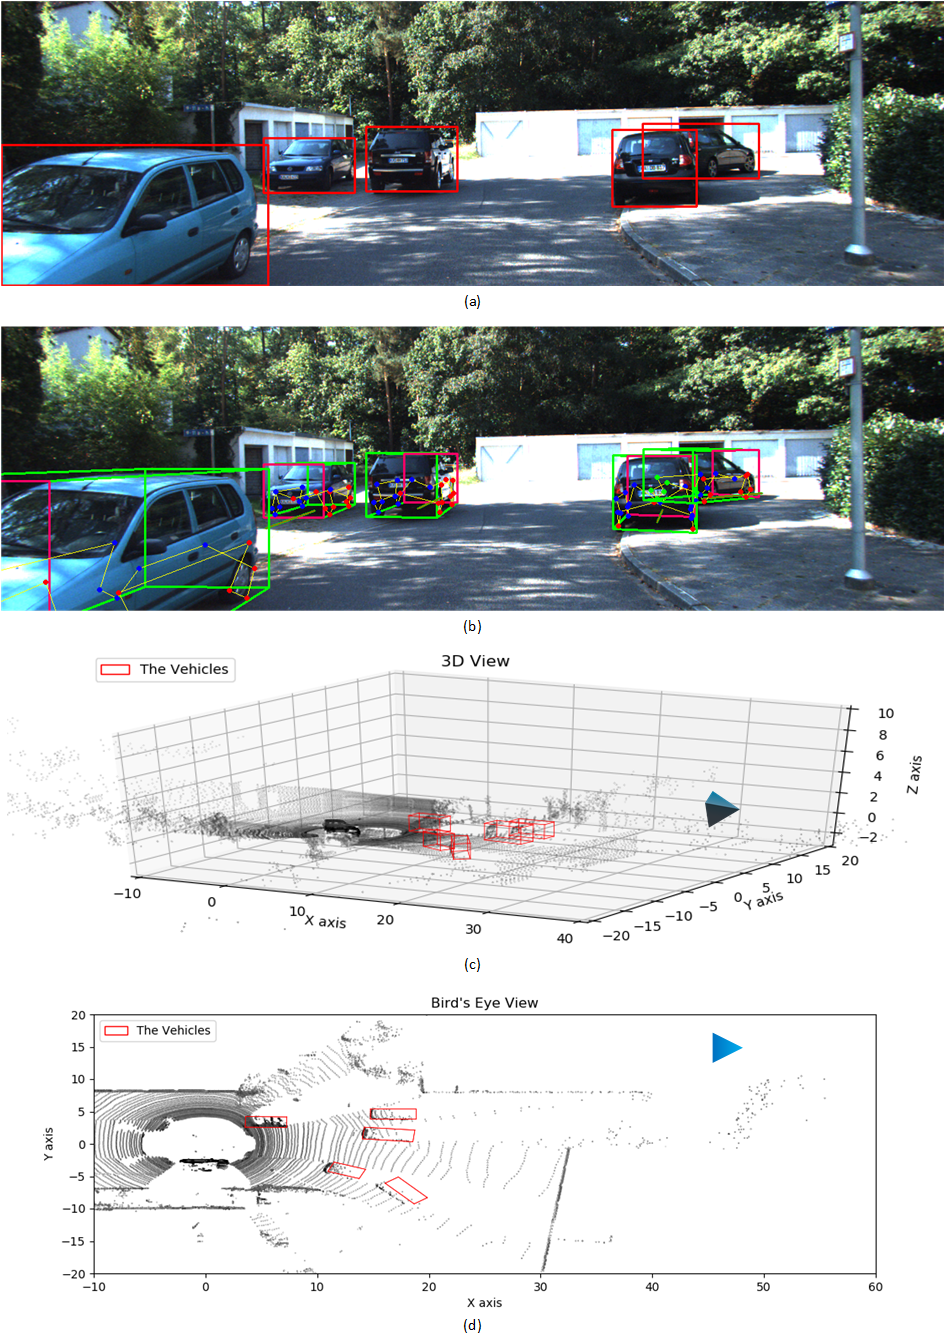
\includegraphics[width=0.9\textwidth]{overall_example.png}
	\caption[Inputs and outputs of our approach.]{Inputs and outputs of our approach: (a). One input KITTI image with 2D bounding boxes for vehicles of interest. (b). The output image with the predicted 3D bounding boxes, 2D parts location, and 2D part visibility property. (c). The estimated 3D bounding boxes in the Velodyne 3D view. (d). The estimated 3D bounding boxes in the bird's-eye view.}
	\centering
	\label{overall_example}
\end{figure}


\subsection{Contributions}

The first contribution of this thesis is a perception learning system that can predict not only the 3D bounding box for each vehicle but also the 3D position of each vehicle part, even if these parts are occluded by other objects or truncated by the image boundaries. The foundation behind this is that vehicles are rigid objects and their geometric characteristics have a lot in common despite the vehicle types. Therefore, these shared geometric characteristics serve as the prior which makes it reasonable that each vehicle can be expressed by a 3D model along with a scaling vector. A 3D model is integrated by vehicle parts which are further encoded by characteristic points. Besides, we apply regression rather than detection to search and locate these characteristic points. By doing so, our approach can find all the parts, as long as it ascertains the existence of the vehicle. Therefore, even though some parts are invisible to the camera, our approach can still localize them. 

The second contribution is the proposed semi-automatic labelling process which generates additional labels to create a new dataset for our approach.  Deep neural networks are greedy for data. Manual labelling is time-consuming and error-prone, let alone it is infeasible to correctly label the distant vehicles or occluded parts in the image. Therefore, we eliminate the human labour to the extent where only the 3D models need to be labelled manually. Then the proposed process automatically selects the best-matching model and projects this model into the real image to generate labels, \eg visibility and characteristic points.  Besides, this process can be easily generalized to other tasks, as long as they require 2D geometry information in the image coordinate system and 3D geometry knowledge in the world coordinate system.

The third contribution is the multi-task framework which includes a prediction neural network and an inference block. The network can simultaneously perform vehicle parts localization, visibility characterization, and dimension proximity prediction at high accuracy level and consequentially, the inference block performs the 3D dimensions estimation,  3D  localization, and 3D orientation estimation for each vehicle. All these tasks can be completed in real time, 0.02s per image, which makes it applicable to directly process the video sequences captured by the front camera of vehicles.

\clearpage

\subsection{Thesis Outline}
First, we present a thorough review of the state-of-the-art methods in 3D object detection relying on different data sources in Section \ref{related_work}. Then in Section \ref{background}, we provide the necessary knowledge and techniques used in this thesis, including autonomous vehicles in Section \ref{avh}, deep learning in Section \ref{dlt}, and computer vision in Section \ref{cv}. Next, we describe our approach in Section \ref{main_work}, the dataset and labelling are presented in Section \ref{data}, the network phase is elaborated in Section \ref{network}, and the inference phase is described in Section \ref{inference}. In Section \ref{exp_eva}, we discuss the design choices of our approach, evaluate our approach on six tasks and compare the results with other methods. Finally, we discuss the deficiencies of our approach and propose possible solutions as future improvements in Section \ref{discussion}.
\clearpage

\section{Related Work}
\label{related_work}
In this section, we present a thorough review of existing works on 3D object detection, especially on 3D vehicle detection, relying on different sensor sources.

\subsection{Mono RGB Image Based Approaches}
Most vehicles are equipped with one monocular camera and RGB images have detailed texture information with high resolution. Therefore, plenty of approaches are developed based on monocular RGB images. Images mainly contain 2D information so most approaches in this category require other help. 

One way is to utilize the geometry information of the vehicles. In this category, a set of algorithms estimate the 3D bounding box based on 3D vehicle models. \cite{834, 741} model the 3D geometry representation of objects with 3D wireframe models. And the 3D bounding box is estimated based on the geometry constraints of the vehicle in the image and its corresponding 3D wireframe model. 3DVP \cite{xiang2015data} performs 3D detection based on 3D Voxel Patterns which are generated from the KITTI dataset \cite{Geiger2012CVPR} and a set of 3D CAD models to encode the geometric information of objects. Mono3D \cite{cvpr16chen} introduces 3D proposals. It exhaustively places 3D bounding boxes on the ground-plane as proposals, then scores each proposal based on several hand-crafted geometric features, and finally applies a CNN to score the most promising candidates to generate the final 3D detections. Recently, CNNs are introduced to estimate some key features for 3D detection. Deep3DBox \cite{DBLP:journals/corr/MousavianAFK16} applies two CNNs to estimate the orientation and dimensions respectively, makes use of the geometric criterion that a 3D box should fit tightly within the 2D box of the vehicle to estimate the translation, and finally integrates them to perform 3D detection. Deep MANTA \cite{DBLP:journals/corr/ChabotCRTC17} performs 3D object detection based on successful 2D object detection. It applies a CNN to predict some 2D key points and the template similarity of the vehicles in images, recovers the corresponding 3D key points and 3D dimensions with some 3D CAD vehicle models, and finally performs 3D detection via 2D-3D matching. Our approach is similar to Deep MANTA in spirit.

Another way is to use temporal information. \cite{7780838, 7298997} make use of motion structure and ground estimation to perform 3D detection from 2D bounding box.


%These approaches are sensitive to the assumptions made and the parameter estimation accuracy so that they perform poorly on the 3D detection task compared to methods that use point cloud data \tbd. whether it's necessary to assess all these approaches.

\subsection{Stereo RGB Image Based Approaches}
A pair of stereo RGB images can provide the depth information of the current scene. 3DOP \cite{DBLP:journals/corr/ChenKZMFU16} recovers depth from stereo images and generates 3D box proposals with the constraints from the depth and other geometry characters, which are forwarded to a modified Fast R-CNN \cite{DBLP:journals/corr/Girshick15} pipeline for object detection and pose estimation. \cite{PHAM2017110} extends 3DOP by applying a separate CNN to extract features from the depth and integrating them for the final 3D detection.


\subsection{Point Cloud Based Approaches}

A LiDAR point cloud is a collection of 3D points acquired by a LiDAR laser scanner. It can represent 3D information of the surroundings but its resolution is lower than that of images.

One set of approaches utilize a point cloud by converting it into a 2D array and making use of the image-based methods to perform 3D detection tasks. This can alleviate the inherent problem that the LiDAR point is often sparse and irregular in 3D voxel representation. VeloFCN \cite{DBLP:journals/corr/LiZX16} projects the point cloud to the front view to generate a 2D point map and then applies a fully convolutional neural network to estimate the 3D bounding boxes for vehicles on this 2D point map. \cite{DBLP:journals/corr/abs-1710-07368, Chen:2015:OPA:2969239.2969287} also fall into this category. Besides, the pre-trained models based on RGB images can be used to initialize the CNNs, which has been proven to be beneficial \cite{DBLP:journals/corr/GuptaGAM14}. However, the 2D representation of LiDAR cloud points suffer from object size variations because of its distance to the sensor and object overlapping.

Another category of approaches transforms the cloud point into a 3D voxel grid representation. Various quantities are used to encode voxels \cite{10.1007/978-3-319-10599-4_41, 7780463, DBLP:journals/corr/Li16p, Wang-RSS-15, DBLP:journals/corr/EngelckeRWTP16}. For example, in \cite{Wang-RSS-15, DBLP:journals/corr/EngelckeRWTP16}, the information in one non-empty cell is encoded with six quantities while empty cells contain no information. For the single-stage detectors, \eg Sliding Shapes \cite{10.1007/978-3-319-10599-4_41} and Vote3D \cite{Wang-RSS-15}, they slide window across the 3D voxel space and apply SVM classifiers to perform 3D detection. To improve the performance, Vote3Deep \cite{DBLP:journals/corr/EngelckeRWTP16} uses a voting strategy with a sparse 3D convolutional network. And \cite{DBLP:journals/corr/Li16p} feeds the point cloud voxel directly to a 3D FCN to generate 3D bounding boxes. For the two-stage framework, \eg Voxelnet, it extends the 2D RPN \cite{DBLP:journals/corr/RenHG015} to 3D to generate 3D proposals and  applies a refine network to score these proposals \cite{DBLP:journals/corr/abs-1711-06396}. 3D CNNs boosts the 3D detection performance while the computation is very expensive and sparsity remains a challenge.  


\subsection{Sensor Fusion Based Approaches}

Images are of high resolution but lack depth, while LiDAR data has 3D information but are sparse and irregular. Thus, many works have investigated combining these complementary data sources together to build robust 3D object detectors. 

One investigated direction is to extract information from these two sources separately for sub-functions. Frustum PointNets \cite{DBLP:journals/corr/abs-1711-08488} first generates frustum point cloud proposals based on 2D object detection, then performs 3D instance segmentation in each frustum point cloud and finally applies a box estimation net to estimate the final 3D bounding box for each object. Similarly, \cite{DBLP:journals/corr/abs-1803-00387} first generates 2D bounding boxes and estimate vehicle dimensions for the target vehicles in images. Secondly, a model fitting algorithm estimates the 3D bounding box on a subset of the point clouds which fall into the 2D bounding box after projection. Finally, a refine 2D CNN performs the final 3D box regression and classification.

The other is to fuse these two kinds of data and process them as a whole. There are various ways to fuse data. One intuitive way is projection. For example, \cite{DBLP:journals/corr/EitelSSRB15} converts the point cloud to a dense depth image and then appends it as an additional channel of the image. \cite{7487370} extends \cite{DBLP:journals/corr/EitelSSRB15} via converting the cloud point to a three-channel HHA map. Their 3D detection score is low mostly due to the loss of 3D information during projection. The more advanced way is to fuse their feature maps. MV3D \cite{DBLP:journals/corr/ChenMWLX16} first generates 3D proposals in LiDAR's bird's-eye view and projects these proposals to the features maps of the image and the bird’s eye view and front view of LIDAR data. Then a deep network fuses three RoI pooling regions and performs 3D detection based on the fused features. PointFusion\cite{DBLP:journals/corr/abs-1711-10871}simultaneously applies a ResNet \cite{DBLP:journals/corr/HeZRS15} to extract appearance and geometry features from image crops defined by the 2D bounding boxes and a modified PointNet \cite{DBLP:journals/corr/QiSMG16} to process the raw point cloud, and finally uses a novel fusion network to integrate both features and estimate 3D bounding box. Recently, Zining \etal \cite{DBLP:journals/corr/abs-1711-06703} apply an innovative sparse non-homogeneous pooling layer to fuse the features extracted from bird’s eye view of LiDAR data and front view camera images by two separate CNNs before region proposal stage. And then a single-stage detector adapted from \cite{DBLP:journals/corr/abs-1708-02002} is designed to perform 3D detection on these fused data without RoI pooling, which is 6 times faster then MV3D. AVOD \cite{DBLP:journals/corr/abs-1712-02294} applies double feature fusions.  It uses two identical CNN to extract features from images and LiDAR data respectively and exploits a Multimodal Fusion Region Proposal Network to generate vehicle proposals from the fused feature crops, projection regions of anchors in the feature maps. Finally, it applies a Multiview Detection Network to perform 3D detection on the fused feature crops corresponding to the proposals. %It achieves the best performance on KITTI 3D vehicle detection up to now.





\clearpage

\section{Background}
\label{background}
\subsection{A Short History of Autonomous Vehicles}
\label{avh}

Autonomous Vehicles (a.k.a. Automated/Driverless/Unmanned/Robotic/Self-driving Vehicles) is a relatively vague concept to the public. Actually, it covers a continuum  from traditional fully human-driving automobiles to fully self-driving vehicles, as SAE classified in Table \ref{figure:loa}.

\begin{table}[h]		
	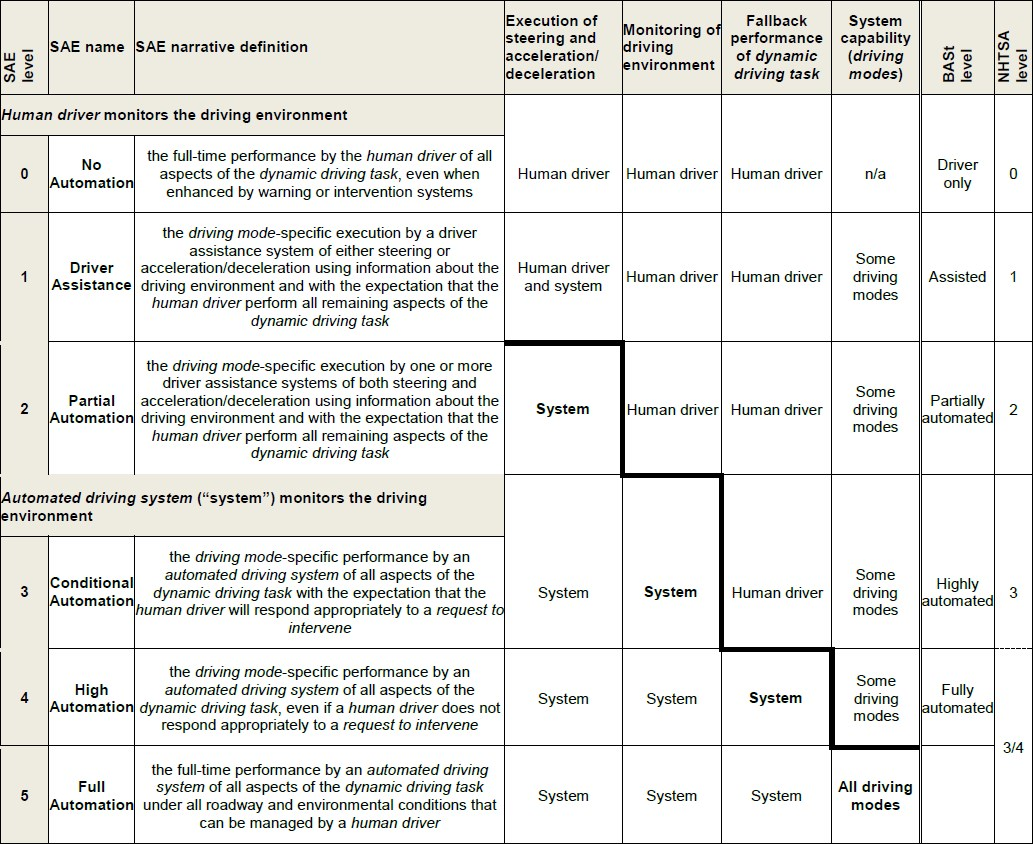
\includegraphics[width=1\textwidth]{Levels_of_Automation_2014.jpg}
	\caption{Summary of levels of driving automation\cite{J3016_201401}.}
	\centering
	\label{figure:loa}
\end{table}

Contrary to the intuition, the idea of Autonomous Vehicles has a long history. The experiments of this fictional idea can be traced back to the 1920s and the technology behind it was radio control \cite{pawtc}. 

But the truly autonomous cars did not show up until the 1980s, even though they could only move slowly on clear streets and required massive human intervention. Mercedes-Benz demonstrated a robotic van based on saccadic vision \cite{schj}. The Autonomous Land Vehicle (ALV) project funded by The Defense Advanced Research Projects Agency (DARPA) cultivated automatic vehicles based on Computer Vision, LIDAR, and autonomous robotic control \cite{Kanade:1986:ALV:324634.325197}. Carnegie Mellon University initially applied a neural network to control the vehicle \cite{NIPS1988_95}. 

In the 1990s, huge progress was made. The VaMP from Daimler-Benz drove more than 1000 km, achieving the maximum speed of 130 km/h on a normal Pairs highway semi-autonomously \cite{schj}. The Navlab project in Carnegie Mellon University achieved a 5000-km journey across America with only 1.8\% human interventions \cite{nohand}. The ParkShuttle in the Netherlands could autonomously navigate itself on a dedicated lane as an automated people mover \cite{parkshuttle}.In this decade, the experiments were mainly carried out in highway scenarios rather than urban scenes.

In the 2000s, competitions promoted this technology a lot. One of the most famous competitions is The DARPA Grand Challenge in the U.S. who offered \$ 1 million for the first prize. In 2004, no vehicle completed the 241-km journey autonomously while 5 teams achieved this goal in 2005 \cite{Buehler2007}. And in Grand Challenge III 2007, known as Urban Challenge, 6 vehicles  finished the event which was a 96-km urban route involving traffic regulations and other vehicles \cite{Buehler2009}.

In the 2010s,  Autonomous Driving Technology starts to take off. Numerous events and projects have been carried out and considerable companies, universities, and research centers have engaged in this field. Based on the progress made before, many autonomous vehicle systems are being tested or even brought into production.  Notable events includes the VisLab Intercontinental Autonomous Challenge in 2010 \cite{doi:10.1504/IJVAS.2012.051250} and the Intelligent Vehicle Future  Challenges from 2009 to 2013 \cite{newlet00}. In industry, Tesla Motor released AutoPilot  that is able to perform automated parking and lane control with autonomous driving, braking and speed adjustment in 2014, and  Audi started the first production car, A8,  reaching Level 3 of Automation in 2017 \cite{historyad}.

Based on the efforts in the last decades, Autonomous Driving is gradually transformed from dream to reality. Its bonus covers safety guarantee, congestion reduction, land use efficiency, energy saving, emission reduction, economic benefits and so on. However, the Level 5 vehicles are so far from maturity that further research and development are in high demand.

\clearpage

\subsection{Deep Learning Technology}
\label{dlt}

Recently, Deep Learning (DL) has shown its impressive power in a variety of tasks, especially in some complex tasks that cannot be explicitly programmed by hand, such as anomaly detection and online advertising. DL delivers the solutions by learning from data automatically via a general learning procedure which dominantly makes use of backpropagation and optimization algorithms, \eg gradient descent.

It attracts world-wide attention mainly by outperforming other classic machine learning algorithms, \eg Support Vector Machine (SVM),  in many competitions in image classification, object detection, or natural language processing. This is because DL applies a deep automatic feature learning architecture, \ie an artificial neural network model with multiple hidden layers, to learn deep distributed hierarchical non-linear representations which yield better performance for learning tasks, \eg in terms of classification accuracy. Such representations bring many good properties, such as feature reuse, parameter sharing,  multiple levels of progressive abstraction, and invariance to local changes of the raw inputs, and thus provide better predictive power than classic machine learning algorithms \cite{6472238}.

Convolutional neural networks (CNNs) is one of the major branches of artificial neural networks. A CNN is a feed-forward multi-layer neural network, typically consisting of one or more convolutional layers,  interleaved by some pooling layers, and finally followed by some fully-connected layers. This modern framework of CNNs is established by LeCun \etal when he proposed the handwritten digit classifier LeNet-5 \cite{726791}. Afterwards, deeper architectures are emerged such as AlexNet \cite{DBLP:Russakovsky14}, VGGNet \cite{DBLP:SimonyanZ14a}, GoogleNet \cite{DBLP:SzegedyLJSRAEVR14} and ResNet \cite{DBLP:HeZRS15}. In general, deeper architectures generate better feature representations and closer approximations to the target function but they also result in more complex models which are more difficult to train and easier to be overfitting. Therefore, many approaches have been proposed to address such problems.

CNNs are specifically designed to work with problems taking images as inputs, such as image classification, object detection and pose estimation. The above-mentioned CNNs examples all made the great performance in their respective tasks, \eg ResNet won the first prize in ILSVRC 2015.

The core building block, convolutional layers, is used to compute feature maps with convolution kernels. Each neuron in a convolutional layer is connected to a local region in the previous layer, called receptive field, and computes an output by performing a convolution operation (element-wise matrix multiplication) between its weights (kernel) and the connected region followed by a non-linear activation function. A nice property of CNNs is that the kernel  is shared by all receptive fields in the preceding layer when computing the corresponding feature map. Thus, each feature map is used to capture exactly the same feature at different locations. And this characteristic can substantially reduce the number of parameters in CNNs, which leads to faster training \cite{nndd}.  

The pooling layers perform a downsampling operation, typically max pooling \cite{Boureau:2010} and average pooling \cite{6460871}, along the spatial dimensions of feature maps to achieve shift-invariance. 

Normally, successive convolution layers detect more abstract features, \eg wheels, than the preceding ones that tend to detect low-level features, \eg curves and edges. Therefore, after the operations performed by several convolutional and pooling layers, progressively higher-level features can be obtained to feed a fully-connected layer whose goal is to perform high-level reasoning to generate the global semantic information \cite{DBLP:SimonyanZ14a, DBLP:abs-1207-0580}.

For classification problems, the output layer of CNNs usually deploys the softmax operator \cite{DBLP:Russakovsky14} or the SVM method \cite{DBLP:Tang13} to output discrete results. Regression tasks, on the other hand, require continuous-valued predictions so that the output layer should have a linear activation function, \eg weighted sum, along with a proper cost function, \eg mean squared error \cite{DBLP:ZhouHSZ16}.

The training for CNNs is a global optimization problem by minimizing the defined loss function. Normally, CNNs can be trained end-to-end efficiently with backpropagation together with an optimization algorithm, such as stochastic gradient descent \cite{5597822}. The mechanism behind it is that gradient of the loss function w.r.t. all parameters are calculated and then used to update the parameters to the direction of minimizing the loss function based on iterations over the full batch or mini batches of the training data.

\clearpage

\subsection{Computer Vision}
\label{cv}

Computer vision is an interdisciplinary field that  enables computers to interpret images just as what we humans can do. Its goal is about automatic extraction, analysis, and understanding of the information from images \cite{BMVA}. There are a huge variety of ways to process images and a marvellous diversity of applications in this board field, ranging from replicating human visual abilities to creating nonhuman visual capabilities \cite{Goodfellow-et-al-2016}. Some real-world applications include object recognition or detection, 3D model building, motion capture, etc \cite{szeliski2011computer}.

Despite all the progress achieved, computer vision systems are still so underdeveloped that they can't match the visual ability against a 5-year-old child. Vision is natural and effortless for humans but factitious and demanding for computers \cite{parallel}. The difficulty in part results from the fact that vision is an inverse problem where we attempt to recover the unknowns, \eg shape and illumination,  based on insufficient information on their causes, \eg models \cite{szeliski2011computer}.  Therefore, it is hard to  explicitly generate  clear problem-solving rules, especially for complex problems, \eg 3D object detection. But currently, Deep Learning seems to find a way out and pushes a big step forward.

Next, in this section, we introduce some basic knowledge in computer vision related to our approach.

\subsubsection{Image Formation}

Imaging systems or cameras are some devices that allow the projection of light from 3D points to a 2D medium that records the light pattern. Figure \ref{figure:camera} (a) shows a pinhole imaging model which is able to capture the light pattern, the inverted candle image, by allowing a very tiny cone of rays issued  at every point of the source, the real candle,  to project on the image plane. This is called pinhole perspective projection which is primitive but provides an acceptable approximation of the imaging process \cite{Forsyth:2002:CVM:580035}. 

The projection equation can be derived from Figure \ref{figure:camera} (b), where $ (O, i, j, k) $ is the pinhole camera coordinate system and the origin $O$ is at the pinhole,  $p=(u, v, d)^T$ is a point in the image, and   $P=(x, y, z)^T$ is a point denotes the source. As light travels straight in the same medium, $p, O$ and $P$ are collinear, and Therefore, we can deduce the Eq. \ref{eq1}: 

\begin{equation}
\label{eq1}
	\begin{cases}
	u = d\frac{x}{z}, & \\    
	v = d\frac{y}{z}   
	\end{cases}
\end{equation}

Modern cameras are built on lenses that can gather more light to make the image more bright while maintaining its sharpness. But the imaging process is very similar to the pinhole camera. Lenses can also introduce some aberrations, \eg spherical aberration, radial distortion, and chromatic aberration \cite{Forsyth:2002:CVM:580035}. Therefore, correction is necessary.

\begin{figure}[h]		
	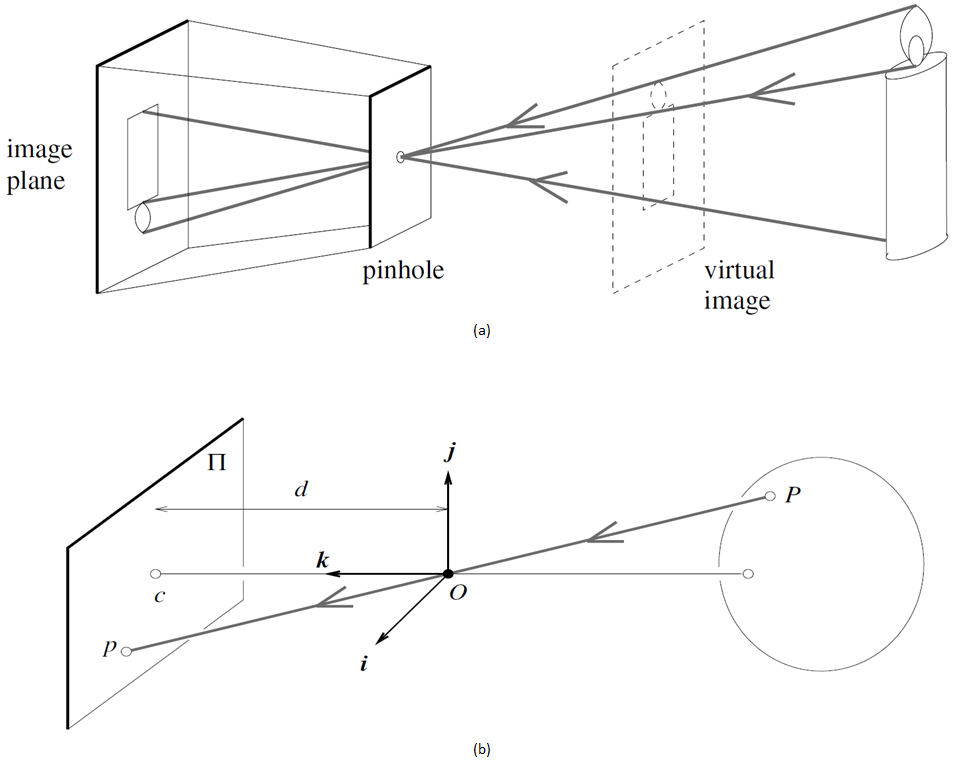
\includegraphics[width=1\textwidth]{camera.png}
	\caption[Pinhole camera model and perspective projection.]{(a). the pinhole imaging model; (b). the geometric model for perspective projection. \cite{Forsyth:2002:CVM:580035}}
	\centering
	\label{figure:camera}
\end{figure}

\subsubsection{Intrinsic and Extrinsic Parameters}
\label{projection}

To project a 3D point in the world coordinate system, we first have to transform this point from the world coordinate system to the camera coordinate system and then transform it into the image plane. The first transformation depends on the extrinsic parameters while the second relies on intrinsic parameters.

\textbf{Intrinsic parameters} include the focal length $f$ just like the $d$ in Figure \ref{figure:camera} (b), the image coordinates origin $(u_0, v_0)$, and the skewed angle $\theta$ of two image axes. Coordinates in the image plane are usually expressed in pixel which can be square or rectangular. So let us assume $\alpha$ and $\beta$ are the value expressed $f$ with horizontal and vertical pixel-meter scales. Therefore, we can finally transform Eq. \ref{eq1} into 
\begin{equation}
\label{eq2}
	\begin{cases}
	u = \alpha \frac{x}{z} - \alpha \cot\theta + u_0, & \\    
	v = \frac{\beta}{\sin\theta} \frac{y}{z} + v_0
	\end{cases}
\end{equation}

When it is written in matrix form as Eq \ref{eq3}, the $3\times3$ matrix $K$ is the intrinsic matrix of the camera. Note that $P^C$ is expressed in camera coordinate system and $P^I$ is in the image coordinate system.

\begin{equation}
\label{eq3}
P^I = K P^C \Leftrightarrow \frac{1}{z}
\bigl(\begin{smallmatrix}
u\\  v \\1
\end{smallmatrix}\bigr) 
= 
\begin{pmatrix}
\alpha & -\alpha \cot\theta & x_0\\ 0 & \frac{\beta}{\sin\theta}  & y_0\\  0 &0  &1 
\end{pmatrix}
\begin{pmatrix} 
x\\  y\\  z
\end{pmatrix}
\end{equation}

\textbf{Extrinsic parameters} define a rigid transformation from world coordinate system to camera frame. A rigid transformation has six degrees of freedom, including three Euler angles expressed in a $3\time3$ rotation matrix $R$ and three translation components along each axis expressed in a $1\times3$ translation vector $t$. A 3D point expressed in homogeneous coordinates is $P=(x, y, z, 1)^T$. Homogeneous coordinates can simplify various geometric transformations into matrix multiplication \cite{Forsyth:2002:CVM:580035}.  Therefore, this rigid transformation expressed in homogeneous coordinates is 
\begin{equation}
\label{eq4}
P^{C} = T_W^C P^W, where ~~T_W^C = 
\begin{pmatrix}
	R & t\\ 
	0^T& 1
\end{pmatrix}
\end{equation}
$P^{C}$ and $P^W$ are coordinates of the same point expressed in world coordinate system and camera coordinate system respectively. $T_W^C$ is the extrinsic matrix of the camera.

To put it all together, the projection equation in homogeneous coordinates is 
\begin{equation}
\label{eq5}
P^I = \frac{1}{z} M P^W = \frac{1}{z} K
\begin{pmatrix}
R & t\\ 
0^T& 1
\end{pmatrix} P^W
\end{equation}
where $M$ is the \textbf{perspective projection matrix}.
\clearpage

\section{Deep3DP Approach}
\label{main_work}
\begin{figure}[h]		
	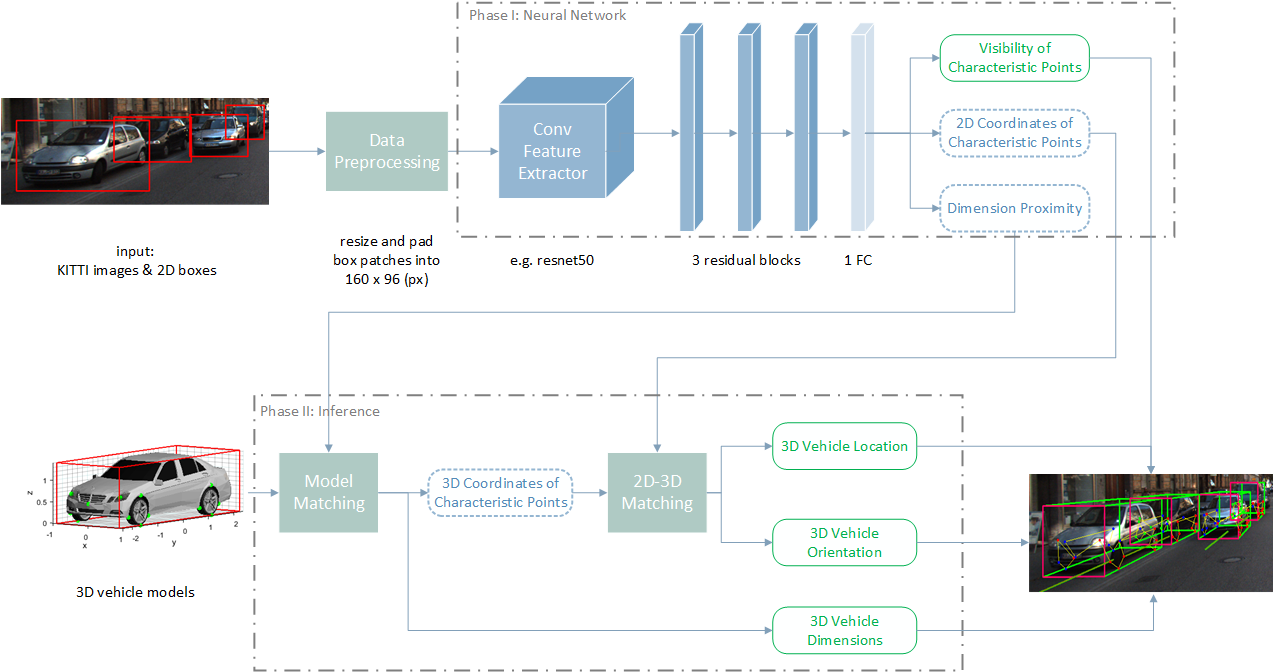
\includegraphics[width=1\textwidth]{app_archi_box_0522.png}
	\caption{The Architecture of our Deep3DP approach}
	\centering
	\label{figure:app_archi}
\end{figure}

In this section, we elaborate on our approach for 3D pose estimation of vehicles in monocular images. Our approach is based on 2D vehicle detection, \ie the 2D bounding boxes of vehicles are given as prior, since 2D object detection techniques, such as YOLO \cite{DBLP:journals/corr/RedmonF16}, Faster R-CNN \cite{DBLP:journals/corr/RenHG015}, SSD \cite{DBLP:journals/corr/LiuAESR15}, R-FCN \cite{DBLP:journals/corr/DaiLHS16}, and FPN \cite{DBLP:journals/corr/LinDGHHB16},  have achieved very high accuracy while 3D object detection performance is still primitive.  The overall architecture of the approach is illustrated in Figure \ref{figure:app_archi}. It consists of two main phases. The first one is the Deep3DP Network which takes the KITTI images and the 2D bounding boxes as inputs and predicts the visibility property and 2D coordinates of all characteristic points, as well as the dimension proximity. The details are presented in section \ref{network}.  The other phase estimates the 3D location, rotation, and dimension of each vehicle based on the 3D vehicle dataset and the outputs of the Deep3DP Network. Section \ref{inference} demonstrated this phase in detail. The KITTI dataset and the 3D vehicle dataset are described in section \ref{data}.


\subsection{Data and Labelling}
\label{data}
\subsubsection{KITTI Dataset}
The KITTI 2D/3D object detection challenge is dedicated to autonomous driving and releases a dataset containing 7481 images for each one of 4 cameras and their associated labels and calibrations \cite{Geiger2012CVPR}. The dataset covers scenarios of City, Residential, Road, Campus, and Person. We only use the images taken by the left colour camera. The example image is shown in Figure \ref{figure:kitti_image}. The associated labels are shown in Table \ref{kitti_lable}. The calibration is given as transformation matrix.

\begin{figure}[H]		
	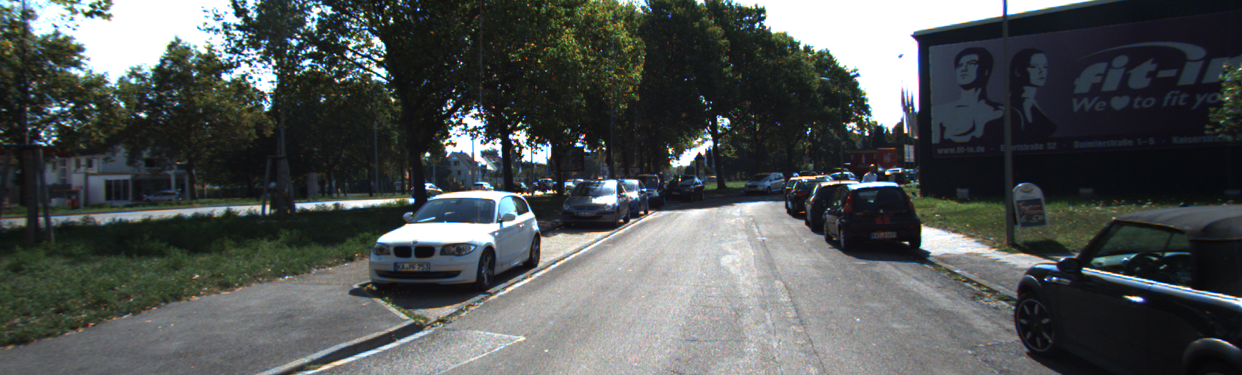
\includegraphics[width=1\textwidth]{000010.png}
	\caption[Example image from KITTI dataset.]{Example image from KITTI dataset captured by the left colour camera.}
	\centering
	\label{figure:kitti_image}
\end{figure}

\renewcommand{\arraystretch}{1.2}
\begin{table}[H]
	\centering
	\caption{Label specification of KITTI dataset}
	\label{kitti_lable}
	\resizebox{\textwidth}{!}{%
		\begin{tabular}{|c|c|l|}
			\hline
			\#Values & Name        & Description                                                                                                                                                             \\ \hline
			1        & type        & \begin{tabular}[c]{@{}l@{}}Type of object: \\ Car, Van, Truck, Cyclist, Tram, Pedestrian, \\ Person\_sitting,  Misc or DontCare \end{tabular}          \\ \hline
			1        & truncated   & \begin{tabular}[c]{@{}l@{}}A float from 0 (non-truncated) to 1,\\ indicating the extent of the object out of the image\end{tabular}                                       \\ \hline
			1        & occluded    & \begin{tabular}[c]{@{}l@{}}An integer indicating occlusion state: \\ 0 = fully visible, 1 = partly occluded, \\ 2 = largely occluded, 3 = unknown\end{tabular}             \\ \hline
			1        & alpha       & Observation angle of the object, ranging {[}-pi..pi{]}                                                                                                                      \\ \hline
			4        & bbox        & \begin{tabular}[c]{@{}l@{}}2D bounding box of the object in the image (0-based index): \\ contains left, top, right, bottom pixel coordinates ($x_1$, $y_1$, $x_2$, $y_2$)\end{tabular} \\ \hline
			3        & dimensions  & 3D object dimensions: height, width, length (in meters)                                                                                                                 \\ \hline
			3        & location    & 3D object location x,y,z in camera coordinates (in meters)                                                                                                              \\ \hline
			1        & rotation\_y & Rotation $r_y$ around Y-axis in camera coordinates {[}-pi..pi{]}                                                                                                           \\ \hline
		\end{tabular}%
	}
\end{table}

\subsubsection{3D Vehicle Dataset}
\label{cad_models}
This dataset is intended to encode the diversity of vehicles according to type, dimension, and chassis shape. It is created based on a selected subset of synthetic 3D CAD models \cite{NIPS2012_4562}. We only include the well-aligned and  symmetrical models, and also take the dimension and type into consideration. We classify all the models into six categories: Mini, Hatchback, Sedan, SUV, Wagon, and Van. And for each category,  subcategories are marked out according to their dimensions and shapes in order to make a refined selection.  The statistic of dimensions is well distributed and each existing vehicle can be classified into one category only.


Our final dataset consists of 54 valid vehicle models. Each vehicle model has a 3D CAD model, a 3D template, and a 3D sketch correspondingly, as shown in Figure \ref{figure:vehicle_dataset}. All these three representations are aligned in canonical view and share an identical object coordinate system. The CAD models are created based on real vehicles and have all the geometry information with them. The 3D templates represent the vehicles' dimensions. The 3D template associated to the 3D model $k$ is denoted as $t_k = (h_k, w_k, l_k)$ where $h_k, w_k$ and $l_k$ represent the height, width, and length of the model respectively. 

The  3D sketches indicate the chassis shapes. Each 3D sketch consists of 20 characteristic points around the chassis with each point denoting one part of the vehicle. So the $k^{th}$ sketch is denoted as $S_k^{3d}  = (p_1, p_2, ... p_{20})$, where $~p_i = (x_i, y_i, z_i)$. The reason why we choose the points around chassis as feature points is that their geometric relationship is more stable than points in other places. Because the chassis part is more about functionality than appearance attraction compared to other parts of the vehicle,  \eg the upper part. In this way, the sketches can be more universal so that they can represent a wider range of vehicles, which reduces the number of models required and further increases the computational efficiency. 

In order to create the 3D sketches, we implement a labelling tool, shown in Figure \ref{figure:label_cad}. It is capable to label the 3D coordinates for all the characteristic points associated to each vehicle. These coordinates are expressed in the object coordinate system.

\begin{figure}[H]		
	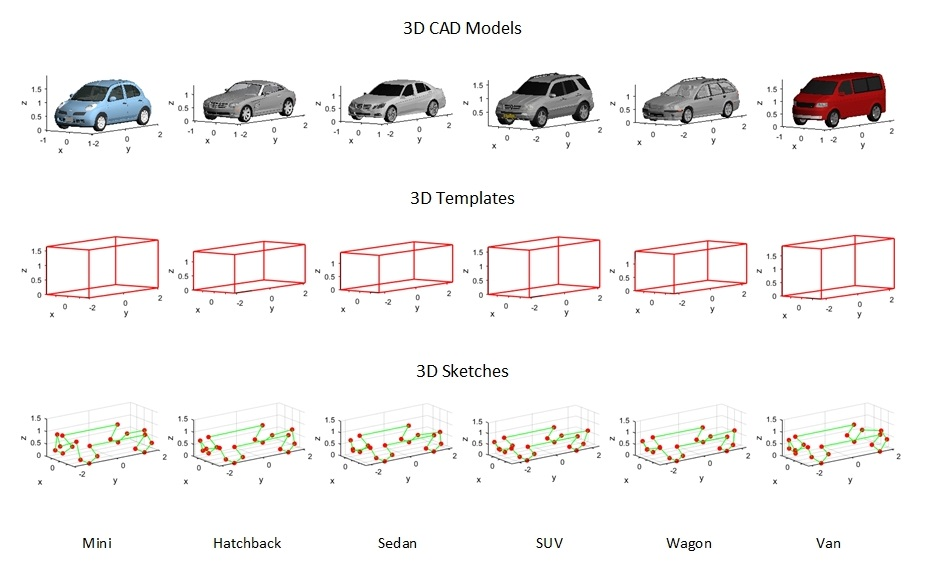
\includegraphics[width=1\textwidth]{vehicle_dataset.jpg}
	\caption[3D vehicle dataset]{Six vehicle categories of the 3D vehicle dataset. Each vehicle model is associated with a 3D CAD model, a 3D template, and a 3D sketch.}
	\centering
	\label{figure:vehicle_dataset}
\end{figure}

\begin{figure}[H]		
	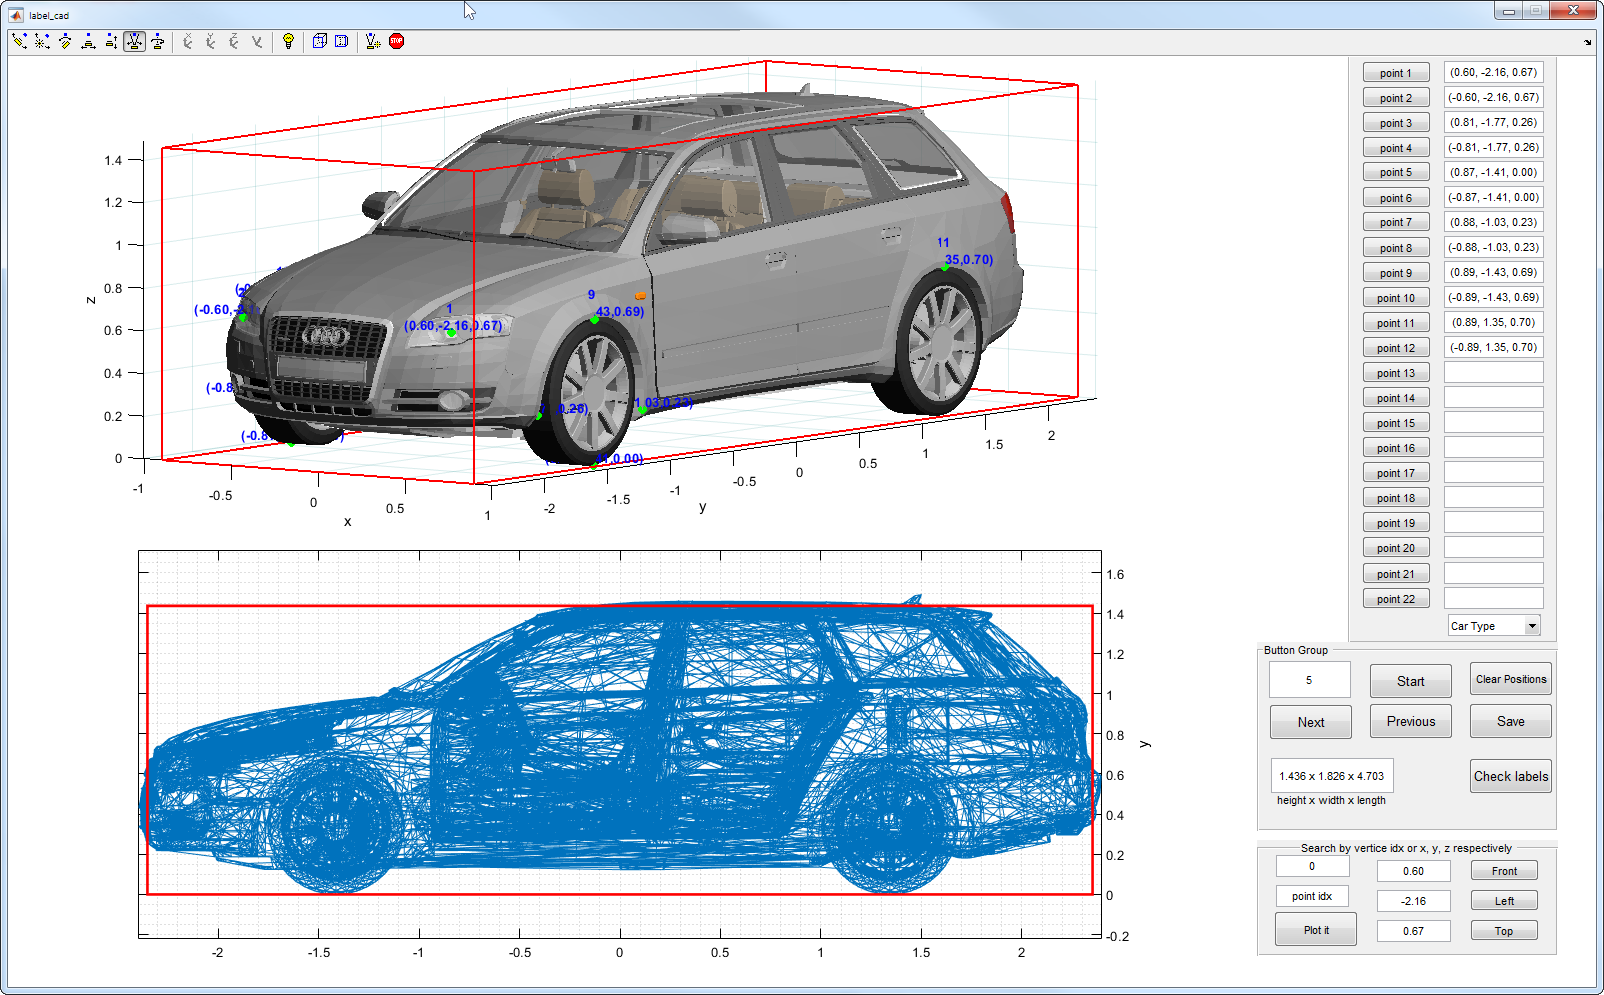
\includegraphics[width=1\textwidth]{label_cad.png}
	\caption{Labelling tool for 3D sketches}
	\centering
	\label{figure:label_cad}
\end{figure}

\subsubsection{Labelling for KITTI Dataset}

Our approach requires three extra kinds of labels to training the Deep3DP Network, \ie 2D coordinates and visibility property of characteristic points and a dimension proximity vector, as shown in Table \ref{new_label}.  Labelling is never a trivial task. Due to the demanding workload of manual labelling and the cases where it is almost impossible to label the small vehicles in the image manually, we propose an automatic label generation method. It is able to make use of the 3D vehicle dataset and the KITTI dataset to generate these three additional kinds of ground truth.

\renewcommand{\arraystretch}{1.2}
\begin{table}[h]
	\centering
	\caption{Specification of three additional labels}
	\label{new_label}
	\resizebox{\textwidth}{!}{%
		\begin{tabular}{|c|c|l|}
			\hline
			\#Values & Name        & Description                                                                                                                                                             \\ \hline
			2x20        & 2D coordinate  & $(x, y)$, the location of 20 characteristic points in the image coordinates                                                                                                                \\ \hline
			1x20        & visibility    & \begin{tabular}[c]{@{}l@{}}An integer indicating visibility property of each point: \\ 0 = visible, 1 = occluded, \\ 2 = self-occluded, 3 = truncated\end{tabular}    \\ \hline
			3x54        & dimension proximity & \begin{tabular}[c]{@{}l@{}} A vector $\mathit{T_{i}}$ represents the dimension ratios \\ between each model and the vehicle  \end{tabular}   \\ \hline
		\end{tabular}%
	}
\end{table}


\paragraph{2D Coordinates}

2D coordinates of key points of each vehicle in the image coordinate system are generated by projecting the 3D sketch of this vehicle to the image. The vehicle's 3D sketch is selected via template-matching, \ie the best-matching sketch is the one whose associated template is closest to the vehicle's dimensions. The 3D-2D projection is performed based on the given intrinsic and extrinsic parameters, as shown in Figure \ref{3D_2D_projection}. The intrinsic parameters are given as calibration by KITTI and the extrinsic parameters are given as 3D object dimensions and rotation $r_y$ in KITTI labels. KITTI makes a simplified assumption here that the vehicle only rotates around the yaw axis but not roll or pitch axis. One example of the labelled 2D coordinates is shown in Figure \ref{visibilie_eg}.

\begin{figure}[H]		
	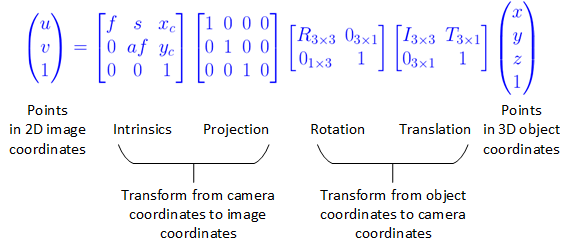
\includegraphics[width=0.8\textwidth]{projection_matrix.png}
	\caption{3D-2D projection}
	\centering
	\label{3D_2D_projection}
\end{figure}

\begin{figure}[H]		
	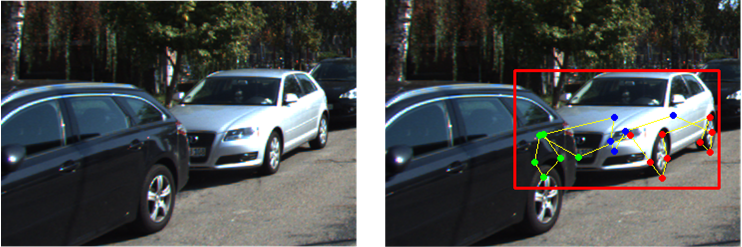
\includegraphics[width=0.8\textwidth]{visibilie_eg.png}
	\caption[Example of 2D coordinates and visibility]{Example of 2D coordinates and visibility of one vehicle. The left image is one patch of KITTI image. The right image is the one after labelling. The points indicate the 2D coordinates and the color indicates the types of visibility: red for visible, green for occluded, and blue for self-occluded.}
	\centering
	\label{visibilie_eg}
\end{figure}

\begin{figure}[H]		
	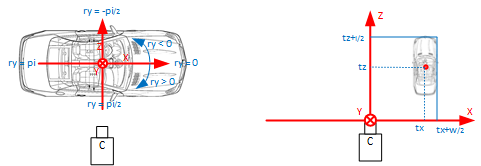
\includegraphics[width=0.8\textwidth]{visibility_imp.png}
	\caption[Visibility labelling mechanism]{Visibility labelling mechanism. The left image shows the rotation $r_y$ in the camera coordinate system, which helps distinguish the visible and self-occluded case. The right image shows the location of the vehicle in the camera coordinate system, which helps define the occluded situation.}
	\centering
	\label{visibility_imp}
\end{figure}



\paragraph{Visibility}
\label{visibility}

As an example of the labelled visibility shows in Figure \ref{visibilie_eg}, the visibility property of characteristic points is classified into four scenarios: 

\begin{enumerate}[\hspace{0.4cm} i.]
	\itemsep-0.5em 
	\item Visible if the point can be seen directly;
	\item Occluded if the point is occluded by other objects;
	\item Self-occluded if the point is blocked out by the vehicle itself;
	\item Truncated if the point exceeds the image boundaries. 
\end{enumerate}


The visibility of each point is determined by its position, \ie the 2D coordinate in the image.  Being visible or self-occluded is distinguished by means of rotation $r_y$ of each vehicle. As the right schematic diagram in Figure \ref{visibility_imp} shows, the rotation $r_y$ can indicate unambiguously which faces of the vehicle are facing to or away from the camera. If the points are on the observable faces, they  are labelled as visible,  otherwise they are classified as self-occluded. Occluded case happens when the 2D coordinate of the point falls into the 2D bounding box of a former object. The object is defined as former when it locates in the region enclosed by the axes and two solid blue line in the left schematic plot of Figure \ref{visibility_imp} if the vehicle is on the first quartile.  And when the vehicle is on the second quartile, it is just a mirrored case. Truncated is identified when the point's 2D coordinate exceeds the image boundaries. The size of KITTI images is determined. The truncated property has the highest priority, the occluded underlies, the self-occluded or the visible is considered at last.


\paragraph{Dimension Proximity}
\label{template}

Dimension proximity of one vehicle is encoded as a vector $\mathit{T_{i}}$ which is defined as $\mathit{T}_i = \{r_k\}_{k \in \{1,.., K\}}$, where $\mathit{K}$ denotes the number of 3D vehicle models and  $r_k~=~(r_h,r_w,r_l)$ corresponds to three scaling ratios between the dimensions (\ie height, width, and length) of each model and the vehicles respectively. The vector $\mathit{T_{i}}$ represents the similarity between each model and the vehicle. The most similar model of a vehicle is the one whose $r_k$ is closest to $(1, 1, 1)$.

\subsubsection{Notations}
In sum, based on the KITTI images and 3D vehicle models, each vehicle can be defined by seven critical attributes:
\[  \{D, B^{2d}, ~B^{3d}, ~C^{2d}, ~C^{3d}, ~V, ~T\}  \]
$D = (h, w, l)$ represents the dimensions of the vehicle. $B^{2d} = (c_u, c_v, w, h)$ defines the 2D bounding box in the image with $(c_u, c_v)$ denoting its centre,  $w$ for its width and $h$ for its height. $B^{3d} = (o, \theta, d)$ where $o = (c_x, c_y, c_z)$ is the centre, $\theta$ is the rotation $r_y$ around the yaw axis, and $d = (w, h, l)$ is its dimensions. $C^{2d}  = \{(u_i, v_i)\}_{i \in \{1, ...,20\}}$ represents the 2D part coordinates in the image plane, while $C^{3d}  = \{(x_i, y_i, z_i)\}_{i \in \{1, ...,20\}}$ denotes the 3D part coordinates in world coordinate system. $V = \{v_i\}_{i \in \{1, ...,20\}}$ is the visibility for all the characteristic points in the vehicle.  $T = \{{(r_{h},r_{w},r_{l})}_k\}_{k \in \{1, ...,54\}}$ is the dimension proximity vector.

\subsection{Deep3DP Network}
\label{network}
This subsection describes the details of the Deep3DP Network, including its architecture, implementation, and training.

\begin{figure}[h]		
	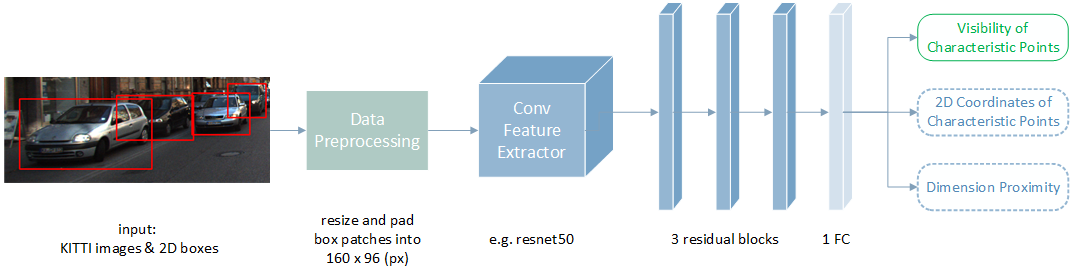
\includegraphics[width=1\textwidth]{NN_archi_box_0522.png}
	\caption{The Architecture of Deep3DP Network.}
	\centering
	\label{figure:nn_archi}
\end{figure}

\subsubsection{Architecture}
The neural network is to learn a map from an $N$-dimensional  input space to an $M$-dimension output space. The map consists of several stages, called layers of the network, written as
\begin{equation}
Y = l_L(...l_2(l_1(X))), \text{where} ~Y \in {\mathbb{R}^M}, ~X \in {\mathbb{R}^N}
\end{equation}

Even though there are various layers, most layers  are composed of neurons, the basic computation element. Most neurons are realized by linear and non-linear operations as 
\begin{equation}
a_{ij} = \sigma(W_{ij}^T X_i +b_j)
\end{equation}

where $a_{ij}$ is the result of the $i_th$ neuron in the $j_th$ layer, $\sigma(\cdot)$ is the activation function and $W_ij$ and $b_j$ are the weights vector and bias applied to input vector $X_i$.  The pooling layer is a special case which performs downsampling operations, such as max pooling \cite{Boureau:2010} and average pooling \cite{6460871}.

As shown in Figure \ref{figure:nn_archi}, our network follows the standard CNN architecture established in LeNet-5 \cite{726791}. It stacks a set of convolutional layers and pooling layers as a feature extractor, followed by 3 residual blocks and one fully-connected layer to refine the features, and three kinds of output layers in the end. The goal of this network is to learn the 2D coordinates and visibility property of 20 interest points and the dimension proximity vector of the vehicle, given the RGB images captured by a monocular camera.

\paragraph{Input Layer}
The input layer accepts the RGB images and feeds them into the network. In theory, images with arbitrary size can be accepted, but to make it more efficient, we use images with fixed size (96 x 160 pixels).  In this way, multiple images can be processed in one batch in order to reduce the variance of parameter updates and make the best use of highly optimized matrix optimizations during training \cite{DBLP:journals/corr/Ruder16}.

Since our approach is based on 2D object detection, each image contains at least one whole vehicle. To obtain these images, we first crop the patches defined by the 2D bounding box, then resize them to match one predefined dimension (96 or 160 pixels), and finally put the resized images in the centre of the 96 x 160 canvas and padded with zeros for other pixel positions. We choose 96 x 160 as the fixed size because they are the means of sizes of all original patches so that we don't have to rescale the patch too much.  Some examples are shown in Figure \ref{figure:patches}.

\begin{figure}[H]		
	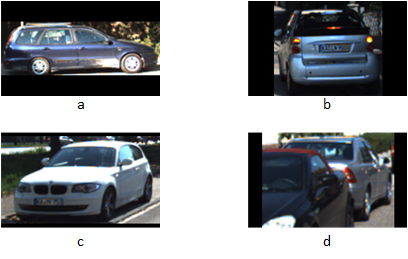
\includegraphics{patches.png}
	\caption[Examples of input images.]{Examples of input images: a. the side view, b. the back view, c. the front view, d. the occluded case}
	\centering
	\label{figure:patches}
\end{figure}

\paragraph{Hidden Layers} 
The hidden layers in Deep3DP network consist of a feature extractor, 3 residual blocks \cite{DBLP:journals/corr/HeZRS15}, and a fully-connected layer. Both the feature extractor and residual blocks are composed of convolutional layers and pooling layers.

The feature extractor is actually one of the available neural network models built in the Keras library \cite{chollet2015keras}, \ie VGG16, VGG19, Xception, ResNet50, \etc  It is trained to  learn deep distributed hierarchical non-linear representations of the input images.

 ResNet50 \cite{DBLP:journals/corr/HeZRS15} is chosen to be the benchmark model because it can ease the training and accelerate the convergence, especially for the fine-tuning. It is well known that there are two main obstacles that hamper the training of deep neural networks: the vanishing/exploding gradient problem \cite{Bengio:1994:LLD:2325857.2328340, pmlr-v9-glorot10a} and the degradation problem that as the network is built deeper, the accuracy gets saturated or even degrades sharply \cite{DBLP:journals/corr/He014}. Residual nets are designed to address these two problems. Instead of learning the direct mapping from input to output, it learns a residual mapping first and then adds the input to it, just as Figure \ref{figure:residual_blocks} (a) shows. The paper validates that it is easier to learn the residual mapping than the direct one and the gradient can always pass through along the short-cut connections. Figure \ref{figure:residual_blocks} (b) and (c) shows two building blocks in our network. (b) is an identity block where the dimensions of input and output matches, while (c) is a linear projection block where the right branch performs $1\times1$ convolution to match the dimensions because the final addition is performed element-wisely.

\begin{figure}[H]		
	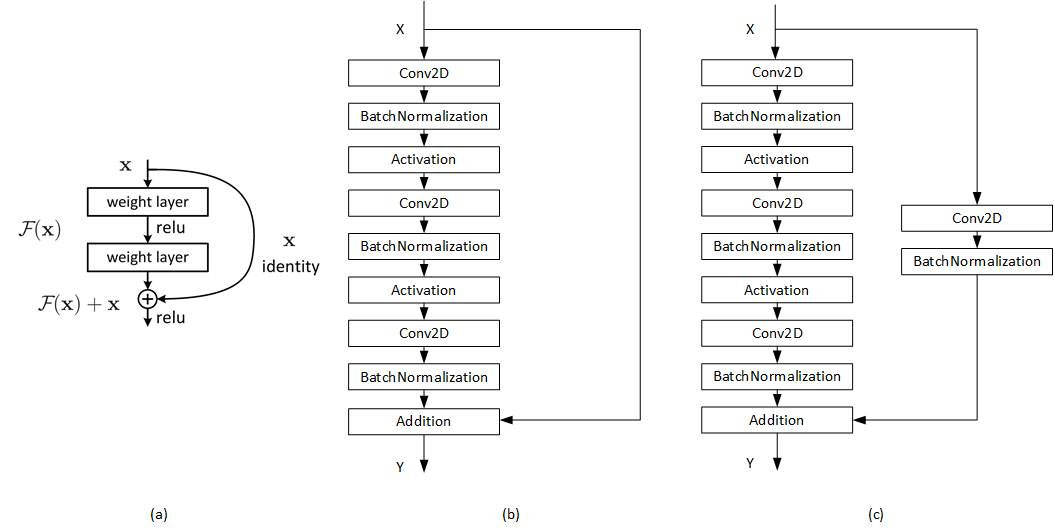
\includegraphics[width=1\textwidth]{residual_blocks.png}
	\caption[Residual network blocks.]{Residual network blocks: (a). a residual block \cite{DBLP:journals/corr/HeZRS15}, (b). an identity residual block in our network, (c). a linear projection residual block in our network}
	\centering
	\label{figure:residual_blocks}
\end{figure}

The last three residual blocks and a fully-connected layer is designed to learn non-linear combinations of the extracted features and then forward them to the output layers.

For all hidden layers, we all apply ReLU as the activation function. The function is

\begin{equation}
\label{relu}
f(z) = \max \{0, z\} ~~~~\text{where}~ z = W^TX+b
\end{equation}

This is a piecewise linear function consisting of two linear pieces, which makes the gradients through a rectified linear unit stay large and consistent whenever the unit is active. Papers \cite{pmlr-v15-glorot11a, Nair:2010:RLU:3104322.3104425, DBLP:journals/corr/JarrettKGL16} have validated that networks activated by ReLU can achieve much better performance than others. ReLU preserves many properties that make it easy for the model to optimize by using gradient-based methods and generalize well, while introducing non-linearity into the model \cite{Goodfellow-et-al-2016}. 

\paragraph{Output Layers} 
\label{output}

Our network has three kinds of output layer for the three tasks respectively. For 2D coordinates regression, a 40-neuron layer with linear activation function is provided.  Each neuron's output indicates one coordinate value, \ie $x_i$ or $y_i$.  20 coordinates are arranged in an ascending order. For visibility characterization, we implement 20 independent quaternary classifiers for 20 points. Each classifier is associated with a softmax activation function \cite{Bishop:2006:PRM:1162264} which outputs four values representing the probabilities of each target class over all possible classes. Dimension proximity is equipped with a 154-neuron linear layer for regression.  Each neuron indicates one ratio element of the dimension proximity vector. Eq.\ref{linear} is a linear activation function while Eq.\ref{softmax} is a softmax activation function.

\begin{equation}
\label{linear}
out_i = W_i^TX_i+b_i
\end{equation}

\begin{equation}
\label{softmax}
out_i = \frac{e^{W_i^TX_i+b_i}}{\sum_{k=1}^K e^{W_k^TX_k+b_k}}
\end{equation}


\subsubsection{Training}

\paragraph{Multi-task Learning}
As mentioned in Section \ref{output}, our network has totally 22 output layers. This implementation makes use of multi-task learning (MTL) where multiple learning tasks are trained in parallel based on the shared features. Caruana has validated that tasks trained in MTL have better generalization performance than trained in a single-task learning mode \cite{Caruana1997}. And he summarizes that this improvement results from leveraging the domain-specific information contained in the training signals of other related tasks \cite{Caruana1997}. Therefore, we follow this paradigm to design our network in order to achieve better performance.

\paragraph{Loss Functions}
\label{loss_functions}
The learning of 2D coordinates and dimension proximity are regression tasks so that a robust smooth $L_1$ loss function \cite{DBLP:journals/corr/Girshick15} is chosen for them. We modify it as

\begin{equation}
\label{eq10}
smooth_{L_1}(x) =
\begin{cases}
~x^2 ~~~~~~~~~~~~~~~~~\text{if} ~\left | x \right |< 0.25 & \\    
~\left | x \right | - 0.1875 ~~~~~\text{otherwise}   
\end{cases} 
\text{where}  ~ x=\widehat{y} - y
\end{equation}
Compared to $L_2$ loss, it is less sensitive to outliers and no special attention is required to pay in order to prevent gradient exploding problem\cite{DBLP:journals/corr/Girshick15}. Besides, when applied with gradient-based optimization, $L_1$ loss and $L_2$ loss often result in poor performance \cite{Goodfellow-et-al-2016}.

For visibility characterization, we develop a model for probabilistic classification so that categorical cross-entropy is used as the loss function. It is also known as the negative log-likelihood \cite{Goodfellow-et-al-2016}, defined as:

\begin{equation}
\label{eq11}
L_{cce} =\frac{1}{N} \sum_{n=1}^N H(y,\widehat{y}) = -\frac{1}{N}\sum_{n=1}^N \sum_{i=1}^c y_{n,i} \log \widehat{y}_{n,i}
\end{equation}

where $H(y, \widehat{y})$ denotes the cross-entropy between the ground truth probability distribution $y$ and the predicted $\widehat{y}$, and $y_{n,i} $ represents the true probability of $i_{th}$ class for the $n_{th}$ data example while $\widehat{y}_{n,i}$ is the estimated. It is a continuous convex loss function which measures the discrepancy between the true and estimated distributions of multi-class classification tasks \cite{DBLP:journals/corr/abs-1802-09941}, which means it can measure the degree of correctness, \ie it can distinguish between ``nearly correct" and ``totally wrong" cases. It outperforms other loss functions in classification tasks and then becomes ubiquitous in deep learning nowadays.

Therefore, training objective is expressed as the total loss of all tasks, written as:
\begin{equation}
\label{eq12}
L_{total} = \lambda_{coord} L_{coord} + \lambda_{temp} L_{temp} + \lambda_{visib}\sum_{i=1}^{20} L_{visib~i}
\end{equation}

where $\lambda_{coord}, \lambda_{temp}$, and $\lambda_{visib}$ are loss weights for these three kinds of tasks respectively. Loss with higher weights has more impact on the gradients and thus tunes the parameters perform better for its corresponding task.

\paragraph{Normalization}
\label{normalization}
Normalization is an important pre-processing step in deep learning which ensures that each feature has a similar data distribution pattern. This is usually done by restricting the features in a certain range or standardizing their ranges. It can enhance the learning capability of the network and speed up the convergence substantially  because it can reduce the bias among features and decrease the low and high-frequency noise in data \cite{Jayalakshmi2011}. The speed-up mechanism can be concluded from Figure \ref{figure:contour}. If we initialize the network at point A in Figure \ref{figure:contour} (a), the gradient-descent update routine will oscillate along the long axis of the eclipse, which definitely takes more time to reach the optimum than any arbitrary initial point in Figure \ref{figure:contour} (b) where the updated trajectory is almost a straight line for any starting point  to the minimum. Besides, this also helps the performance because the updated trajectory oscillates less around the minimum for case (b) than case (a) so that it is more likely for case (b) to reach the optimum.

\begin{figure}[h]		
	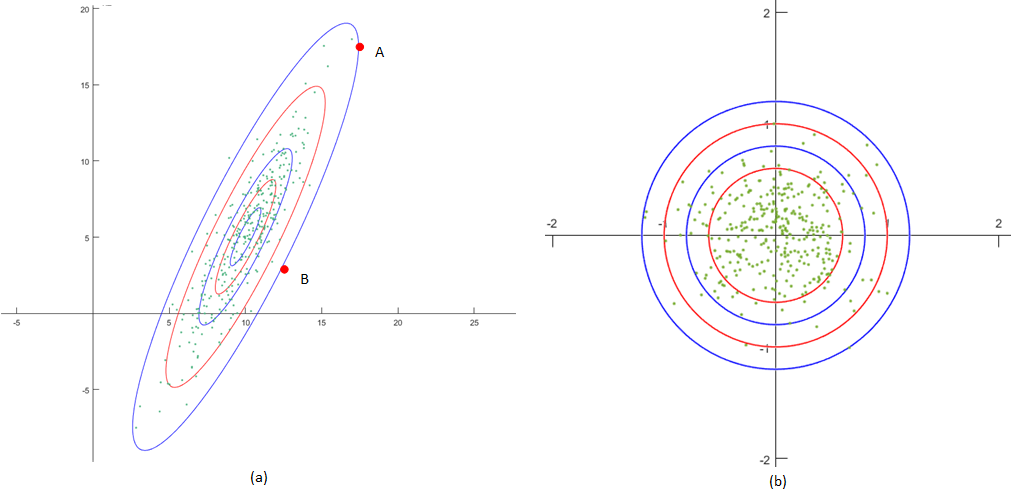
\includegraphics[width=1\textwidth]{contour.png}
	\caption[Effect of nomalization.]{Effect of normalization: (a). data distribution before normalization, (b). data distribution after normalization}
	\centering
	\label{figure:contour}
\end{figure}

Our network takes RGB images as input so that pixel intensity is the input feature. The technique we use to normalize the image is channel mean subtraction, used in \cite{DBLP:journals/corr/SimonyanZ14a, DBLP:journals/corr/GirshickDDM13}, which centers all the features around the origin along each dimension. As mentioned in CS231N \cite{CS231N}, mean channel subtraction is enough for CNNs and the original range of pixel values is determined, \ie $[0, 255]$.

The range of ground truth influences the loss. In order to make the three types of labels impact similarly on the loss, we normalize them. For visibility, we use one-hot-encoding to encode its classes so that it only has value 0 or 1. The value of 2D coordinates $C^{2d}  = \{p_1, p_2, ...,p_{20}\}$varies greatly so that we normalize them w.r.t. the associated 2D bounding box $B^{2d} = (c_u, c_v, w, h)$ \cite{DBLP:journals/corr/ChabotCRTC17}. The normalized 2D coordinates $\overline{C}^{2d}  = \{\overline{p}_1, \overline{p}_2, ...,\overline{p}_{20}\}$ ranges $[-1, 1]$, where
\begin{equation}
\overline{p}_i  = (\frac{u_i - c_u}{w}, \frac{v_i - c_v}{h})
\end{equation}

The dimension proximity vector $T$  is normalized with $\log$ function element-wisely \cite{DBLP:journals/corr/ChabotCRTC17}, resulting in $\overline T$ and its range falls into $[-1, 1]$, too.

Moreover, as Sergey \etal \cite{DBLP:journals/corr/IoffeS15} state the variation of each layer's input distribution during the training makes the training complicated and hard to converge quickly so that we apply Batch Normalization (BN) to alleviate the internal covariate shift phenomenon.  BN normalizes the summed activations of each layer to a distribution of zero mean and unit variance. The mean and variance of each activation are computed on each mini-batch. By doing so, much larger learning rate can be used for training and no special attention has to pay on parameter initialization. 
 
\paragraph{Regularization}
Regularization techniques are used to address the overfitting problem in order to make an algorithm not only perform well on the training data but also on the test data, the previously unseen data \cite{Goodfellow-et-al-2016}. Overfitting results from either that the algorithm is too complicated for the data or that the sampled data is not able to represent the internal pattern. Normally, we design an algorithm to model  the data pattern exhaustively first and then apply regularization techniques to make the algorithm generalize well.  

In the data aspect, we use data augmentation as a regularization. The best way to address overfitting is to train the model on more data, but the amount of data is restricted for one dataset. Therefore, we generate some synthetic data. Since our network involves classification and regression tasks, we mainly enlarge the dataset via horizontal flipping and scaling. 

In the architecture aspect, Batch Normalization \cite{DBLP:journals/corr/IoffeS15} is used as the regularization in each layer. BN enables the network to obtain the information of the training sample and the others in mini-batch simultaneously so that it does not generate deterministic dependency on this training sample. Therefore, BN can replace Dropout \cite{JMLR:v15:srivastava14a} to be the regularization for our convolutional network. 

Besides, Multitask Learning is another technique we used to improve generalization performance. In our network, the learning representation is shared across all tasks so that the parameters shared are constrained from biasing towards one specific task, \ie only the representation that is useful for more than one tasks can be kept \cite{Goodfellow-et-al-2016}.  Therefore, the statistical strength of the parameters is highly enhanced \cite{Baxter:1995:LIR:225298.225336}.

During the training, early stopping is applied to prevent the model being trained too complex to fit the test data. As Figure \ref{figure:optimization} (a) shows, we halt the training when the validation error stops decreasing.  The stopping point is when the learned model can represent the pattern of validation data most. It regards the number of training epochs as a hyperparameter and can effectively tune it to be optimal \cite{DBLP:journals/corr/abs-1206-5533}  because early stopping can restrict the global learning capacity of a large network to fit simpler dataset without affecting the backpropagation to control the learning capacity locally \cite{Caruana:2000:ONN:3008751.3008807}.


%\begin{figure}[h]		
%	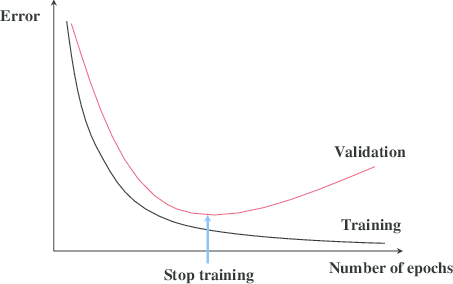
\includegraphics{early_stopping.png}
%	\caption{Early stopping}
%	\centering
%	\label{figure:early_stopping}
%\end{figure}

\paragraph{Parameter Initialization}

Transfer learning is proposed to transfer the representation learned from one task to another related task \cite{Pan:2010:STL:1850483.1850545}. As it is known that CNNs learn more abstract features in a deeper layer. It is not surprising to find that, for visual tasks, shallow layers learn low-level features, \eg edges, corners, changes in lighting, \etc, which are shared across datasets and tasks. Moreover, Yosinski \etal validate \cite{DBLP:journals/corr/YosinskiCBL14} that initializing a network with transferred features can improve the generalization capability hugely and Yoshua \etal \cite{NIPS2006_3048} confirm that this initialization put the start point closer to a local minimum than random initializations, resulting in accelerating convergence.

Therefore, we initialize our feature extractor with parameters learned on ImageNet dataset \cite{DBLP:Russakovsky14} and the three residual blocks with parameters trained on the KITTI dataset. The fully-connected layer is initialized from a zero-mean Gaussian distribution with standard deviation 0.01 and all the output layers are initialized with zeros.


\paragraph{Learning Algorithms / Optimization}

Optimization is a task of finding the value $x$ in order to minimize or maximize some objective function $f(x)$. One most powerful optimization technique category in deep learning is gradient-based.

As it is known, the derivative $f'(x)=\frac{\text{d}y}{\text{d}x}$ specifies how to make a small change $\epsilon$ of the input $x$ to get the corresponding change in the function:
\begin{equation}
	f(x + \epsilon)~ \approx ~ f(x) + \epsilon f'(x).
\end{equation}

Thus, the derivative tells the direction to minimize a function, i.e. it can point out how to change $x$ to make a small update. One popular algorithm, gradient descent \cite{gd1847}, makes use of the derivatives and update the input $x$ directly as:

\begin{equation}
x = x - \alpha {\triangledown} _x f(x)
\end{equation}

where $\alpha$ is the learning rate, a positive real value to decide the size of an update step. The examples in Figure \ref{figure:optimization} (b) show how the update works.  A deep network often consists of many layers so that back-propagation algorithm \cite{Rumelhart:1988:LRB:65669.104451} is used to compute the gradient for each parameter in different layers of the objective function based on the chain rule of calculus.

\begin{figure}[h]		
	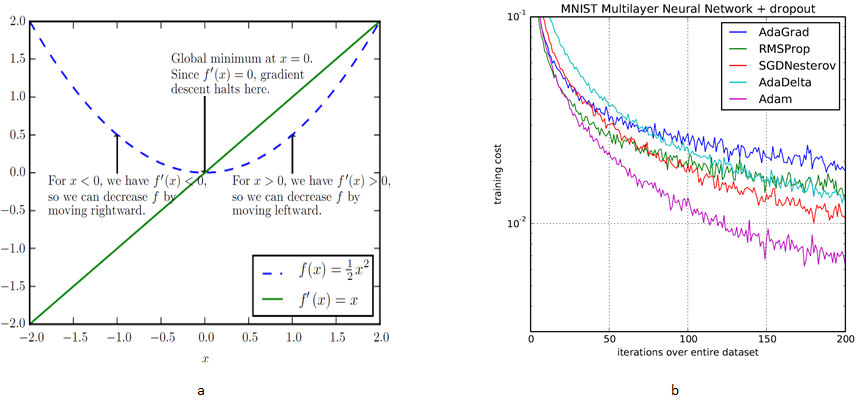
\includegraphics[width=1\textwidth]{optimization.png}
	\caption[Optimization]{(a). Early-stopping during the training. (b). examples showing how gradient descent makes use of derivatives to reach a minimum \cite{Goodfellow-et-al-2016}, (c). performance of optimization algorithms in the same setting \cite{DBLP:journals/corr/KingmaB14}}
	\centering
	\label{figure:optimization}
\end{figure}

In deep learning, the input of the objective function is often multidimensional so that it probably has many local minima and saddle points, which renders huge difficulties to optimization. Therefore, we usually take in a compromise scenario where the value $x$ makes $f$ really low but not necessarily globally minimal \cite{Goodfellow-et-al-2016}.

The optimization algorithm we used is Adam \cite{DBLP:journals/corr/KingmaB14} which is robust and efficient in memory and computation for the optimization of stochastic objectives in a high-dimensional parameters space. It makes use of both the gradient and its momentum to update parameters as: 

\begin{algorithm}[H]	
	\While{$x_t$ not converged}{
		$ t = t + 1 $\;
		$ g_t = {\triangledown} _x f(x_{t-1}) $\;
		$ m_t = \beta_1 m_{t-1} + (1-\beta _1) g_t$ \;
		$ v_t = \beta_2 v_{t-1} + (1-\beta_2) g_t^2 $\;
		$ \hat{m}_t = \frac{m_t}{1 - \beta _1^t} $\;
		$ \hat{v}_t = \frac{v_t}{1 - \beta_2^t}  $\;
		$ x_t = x_{t-1} - \alpha \frac{\hat{m}_t}{\sqrt{\hat{v}_t} + \epsilon}$\;
	}
	%\caption{Adam algorithm update mechanism}
\end{algorithm}

where $ t $ denotes the current iteration, $\alpha$ is the learning rate, $\beta_1$ and $\beta_2$ are two exponential decay rates, and $\epsilon$ is a small scalar to prevent zero-division.

From the Figure \ref{figure:optimization} (c), we can see that Adam can make the learning task converge relatively faster and has lower training error. Thus, we follow this guide to apply Adam to our optimization of Deep3DP Network.

\subsection{Inference}
\label{inference}

As shown in Figure \ref{figure:inference}, the inference phase consists of two main steps: template matching to obtain the 3D coordinates of characteristic points and 3D dimensions for the objective vehicle and 2D-3D matching to recover the 3D vehicle location and rotation.

\begin{figure}[h]		
	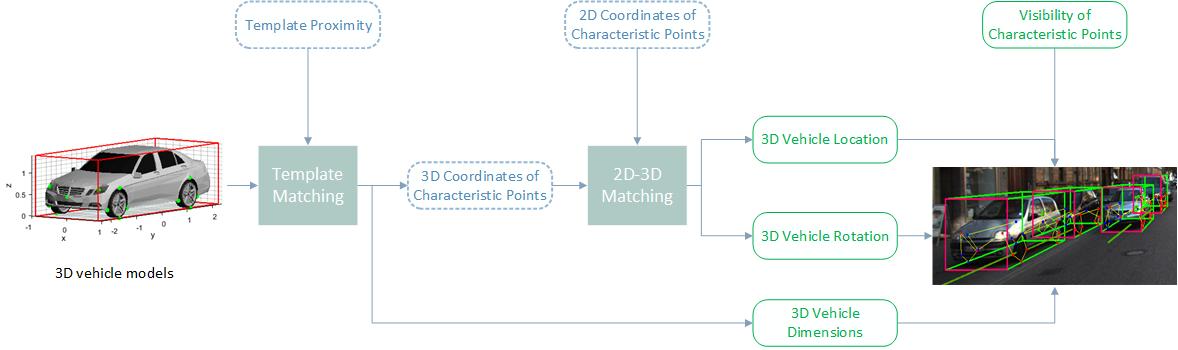
\includegraphics[width=1\textwidth]{inference_0522.png}
	\caption{The Architecture of our Approach}
	\centering
	\label{figure:inference}
\end{figure}

\subsubsection{Template Matching}

Template matching is based on the 3D template dataset and the learned dimension proximity for the objective vehicle in the image. As defined in section \ref{template}, dimension proximity vector, ${T} = \{{(r_h,r_w,r_l)}_k\}_{k \in \{1,.., K\}}$, measures the dimension similarity between the target vehicle and 3D vehicle models. The best matching model is the one whose dimensions $(h, w, l)$ has the least distance to the target vehicle's dimension $(\bar{h}, \bar{w}, \bar{l})$, \ie the corresponding scaling ratios, $(r_h,r_w,r_l)$, is closest to $(1, 1, 1)$. 

Let us denote the best matching template for the target vehicle $m$ as $t_j$ and the dimension ratio between the target vehicle and the best matching model as $r_j = (r_h,r_w,r_l)$. Then its corresponding 3D sketch is $S_j^{3d}  = (p_1, p_2, ... p_{20})$. To get the target vehicle's dimension $D_m$, we apply the scaling ratios, $(r_h,r_w,r_l)$, to $t_j$ as
\begin{equation}
	D_m = t_j \cdot r_j =  (h_j, w_j, l_j) \cdot (r_h,r_w,r_l) = (h^m, w^m, l^m)
\end{equation}

In the same way, we can get the 3D coordinates of the interest points of the objective vehicle, $C_m^{3d}$, as
\begin{align}
C_m^{3d} &= S_j^{3d} \cdot r_j \nonumber \\  
					  &=  {\{(x_i, y_i, z_i)\}}_{i \in \{1, ...,20\}} \cdot (r_h,r_w,r_l) \nonumber \\  
					  &= {\{(x_i^m, y_i^m, z_i^m)\}}_{i \in \{1, ...,20\}} \qquad {} 
\end{align}

\subsubsection{2D-3D Matching}

Based on the projection mechanism described in section \ref{projection}, the 2D coordinate of one point in the image coordinate system can be generated via projecting the 3D point in the world coordinate system with the perspective projection matrix to the image plane. This process is described in Figure \ref{3D_2D_projection}. Now the Deep3DP network predicts the 2D coordinates, $C_m^{2d}$, of the 20 interest points of the target vehicle $m$ and the template matching process provides the corresponding 3D coordinates, $C_m^{3d}$. Then the 3D-2D projection equation in homogeneous coordinates becomes:
\begin{equation}
	C_m^{2d} =   K_{3\times 4}
	\begin{pmatrix}
	R_{3\times 3} & t_{3\times 1}\\ 
	0_{1\times 3}& 1
	\end{pmatrix} C_m^{3d}
\end{equation}

where $K_{3\times 4}$ is the given camera calibration matrix, $R_{3\times 3}$ and $t_{3\times 1}$ are the rotation and translation to be computed. Figure \ref{figure:corresp} shows the 2D-3D correspondence points for each vehicle and its model. It is easy to compute the rotation and translation of the target vehicle in the camera coordinate system with the standard 2D-3D matching algorithm, \ie EPnP \cite{Lepetit2008}. Its central idea is that each of the $n$ reference points can be expressed as a weighted sum of four virtual control points, which makes these control points as the unknowns instead of the original $n$ points. Based on this, it can use the 3D-2D projection property to find a pair of rotation matrix and translation vector that minimize the reprojection error non-iteratively, as shown in Eq. \ref{Rt}:

\begin{equation}
\label{Rt}
	R, t = \underset{R,t}{argmin}\sum_i dist^2(K[R|t]\begin{bmatrix} C_m^{3d} \\1  \end{bmatrix}_i, ~ (C_m^{2d})_i)
\end{equation}

The KITTI data simplifies the rotation to one dimension, $r_y$, so that we follow this convention. Translation is the 3D coordinate of the origin of the vehicle so that it can represent the location of the vehicle in the camera coordinate system.

\begin{figure}[H]		
	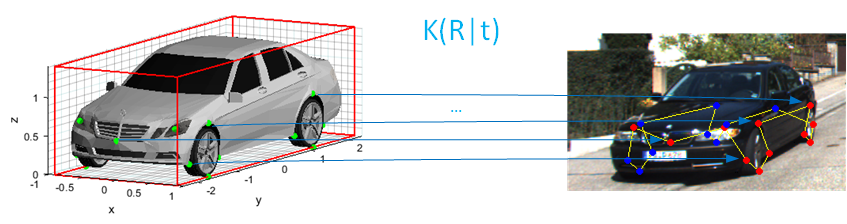
\includegraphics[width=0.8\textwidth]{corresp.png}
	\caption[Example of 2D-3D correspondence points.]{Example of 2D-3D correspondence points. Left: $C_m^{3d}$ in object coordinate system. Right: $C_m^{2d}$ in the image.}
	\centering
	\label{figure:corresp}
\end{figure}

\begin{figure}[H]		
	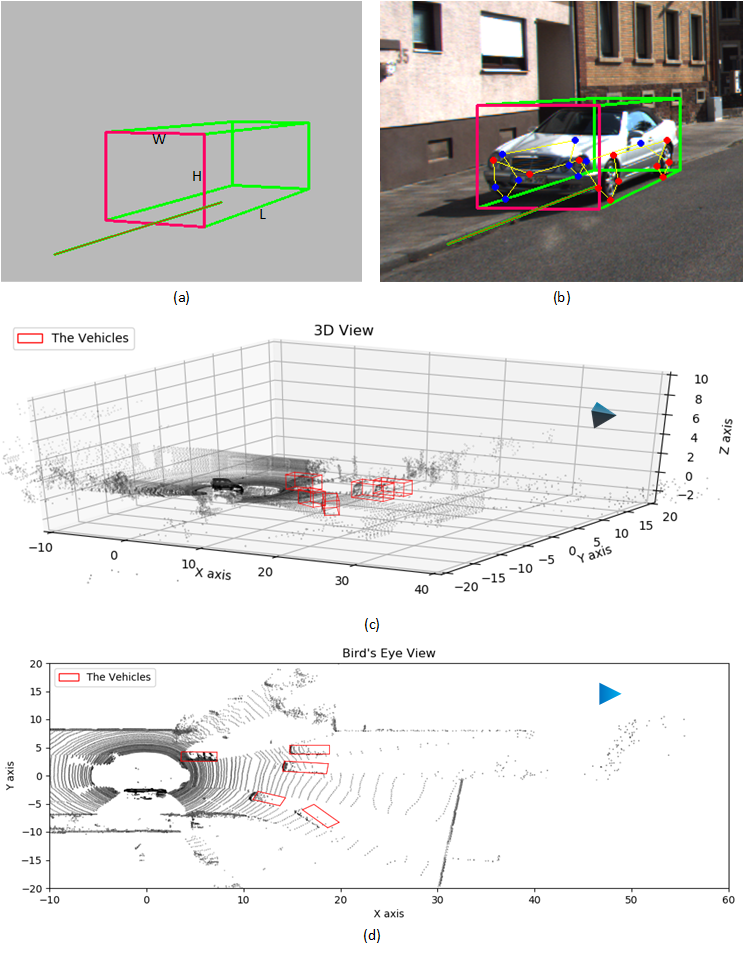
\includegraphics[width=0.8\textwidth]{visualization2.png}
	\caption[Visualization of the outputs of our approach]{(a). Visualization sketch of 3D bounding box and orientation, (b). Visualization of the 3D bounding box, key points, and their visibility. (c). 3D visualization in the Velodyne 3D view, (d). 2D visualization in bird's-eye view.}
	\centering
	\label{figure:visualization}
\end{figure}


\subsubsection{Visualization}
To visualize the 3D bounding box, we use the vehicle's dimensions to determine the eight corners of the cuboid and then project this cuboid into the image with the projection matrix which is composed of the recovered rotation and translation. And in order to show the rotation clearly, we project a line on the ground to show the direction of the vehicle. This visualization mechanism is shown in Figure \ref{figure:visualization} (a) where the front face of the vehicle is coloured with magenta. Figure \ref{figure:visualization} (b) shows a example of this visualization. 

Besides, to better visually check the performance of our approach, we visualize the estimated 3D bounding boxes in 3D view and bird's-eye view. Figure \ref{figure:visualization} (c) shows an example in 3D view where we plot the 3D bounding boxes in the cloud points of the current frame and the pyramid denotes the forward direction. Figure \ref{figure:visualization} (d) shows an example in bird's-eye view where we can clearly illustrate the location of vehicles.





\clearpage

\section{Experiment and Evaluation}
\label{exp_eva}
In this section, we first describe the experiment setup and evaluation metrics in Section \ref{setup} and \ref{eval_met}. Second, we discuss the most crucial design choices for our approach in Section \ref{d_choices}. Finally, we evaluate our approach and its variations, and compare our approach with the start-of-the-art methods on monocular 3D pose estimation of vehicles in Section \ref{exp_res}.

\begin{figure}[H]		
	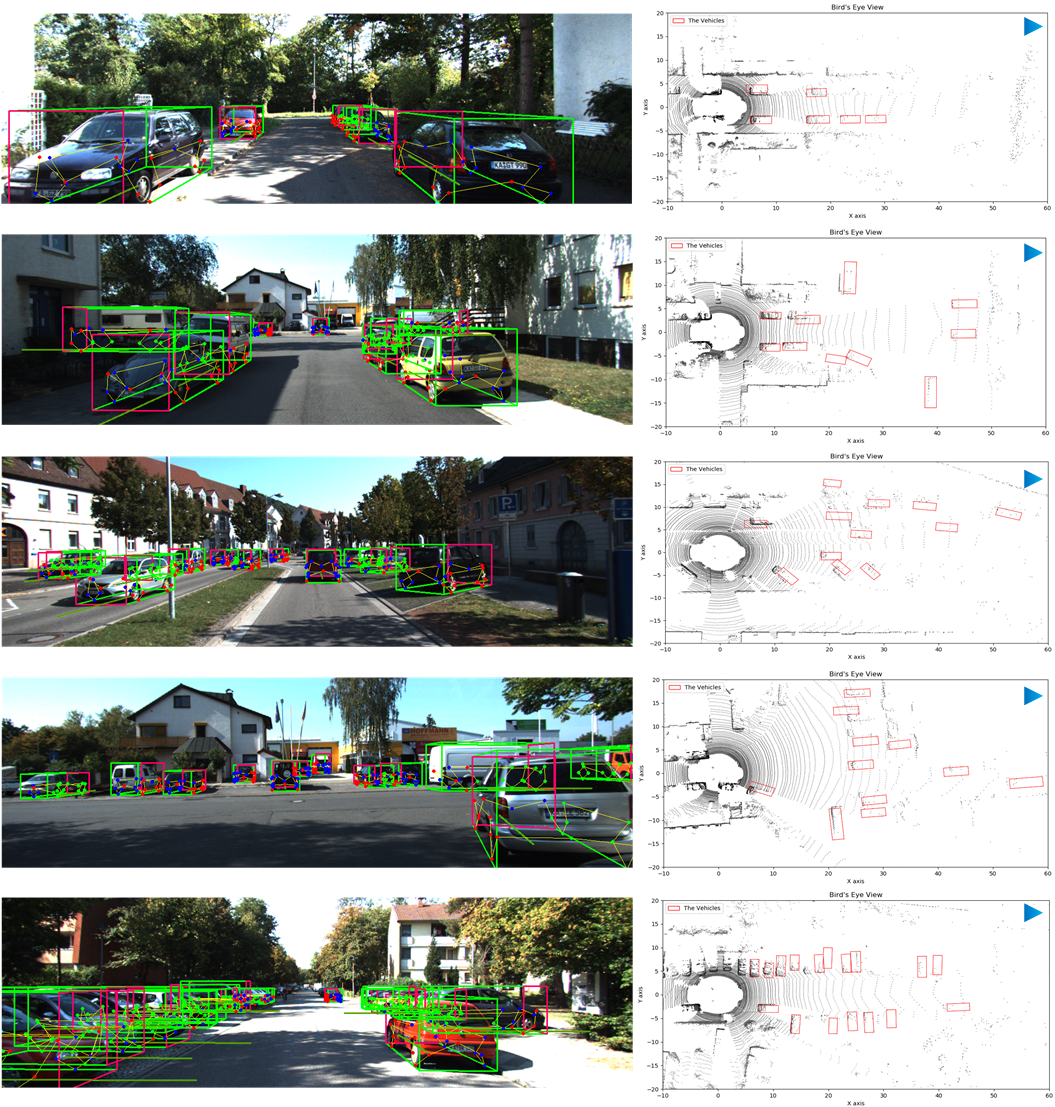
\includegraphics[width=0.98\textwidth]{res_img2.png}
	\caption[Examples of the output images of our approach.]{Examples of the output images of our approach. Image outputs are on the left. bird's-eye view outputs are on the right.}
	\centering
	\label{figure:res_img}
\end{figure}

\subsection{Experiment Setup}
\label{setup}

We have presented the approach in Section \ref{network} and \ref{inference} which is served as a baseline model of our approach. Some other design choices are made based on it. The benchmark network uses ResNet50 \cite{DBLP:journals/corr/HeZRS15} as feature extractor, initialized with pre-trained weights trained on ImageNet \cite{DBLP:Russakovsky14}, and is trained with Adam \cite{DBLP:journals/corr/KingmaB14}. The network is implemented on Keras \cite{chollet2015keras} using TensorFlow \cite{tensorflow2015-whitepaper} as backend. Keras supports running both on GPU and CPU. 

We evaluate our approach and its variations on the dataset created based on KITTI 3D object detection benchmark \cite{Geiger2012CVPR}, described in Section \ref{data}. Because the KITTI only releases the ground truth for 7481 training images, we split them into train and validation set for training and validation respectively. We follow difficulty division policy of  KITTI and extend to more detailed levels. We use 54 vehicle CAD models \cite{NIPS2012_4562} for semi-automatic labelling and template matching. Each model is encoded with 20 points for its corresponding 3D sketch.

We evaluate six tasks: 3D bounding box estimation, orientation estimation, 3D localization, 3D dimension estimation, 2D part localization, and 2D part visibility prediction. 3D bounding box estimation is the ultimate task, representing the localization, orientation, and dimension of the 3D bounding box,  which is Therefore, used to assess all the design choices.
\subsection{Evaluation Metrics}
\label{eval_met}

We use intersection over union (IoU) to measure the performance of 3D vehicle detection. IoU is used to measure the similarity of 2D bounding boxes in various 2D object detection challenges, \eg Pascal VOC \cite{Everingham15} and ILSVRC \cite{DBLP:Russakovsky14}. It is extended to measure 3D object detection with the formula:
\begin{equation}
	IoU(b_1, b_2) = \frac{V(b_{pre}\cap b_{gt})}{V(b_{pre}\cup b_{gt})}
\end{equation}
where $V(\cdot)$ indicates the volume and $b_{pre}$ denotes the predicted 3D bounding box while $b_{gt}$ is the ground truth. KITTI 3D object detection benchmark considers that a 3D bounding box estimation is correct, if $IoU \geq 0.7$ \cite{Geiger2012CVPR}. If multiple bounding boxes are predicted for one vehicle, they are considered as false predictions. %{But in our experiment, we lower the criterion to $IoU \geq 0.5$.}% 

For 3D orientation estimation, we use the measure, Orientation Score (OS), defined in \cite{DBLP:journals/corr/MousavianAFK16}. It is the mean score across all estimations in the validation set, written as:
\begin{equation}
	OS =\frac{1}{N} \sum_{i=1}^N\frac{(1+\cos(\triangle \theta_i))}{2}
\end{equation}
where $N$ denotes the number of examples in the validation set and $\triangle \theta_i$ represents the difference between the predicted orientation $r_y$ and the ground truth for example $i$.

 For other tasks, we follow the metrics defined in \cite{DBLP:journals/corr/ChabotCRTC17}. A 3D localization is considered correct if its distance to the ground truth is less than a threshold. Two thresholds, 1 meter and 2 meters, are chosen. 2D part localization is measured the same way and the threshold is 20 pixels. 3D dimension estimation is correct if the predicted dimensions $(h, w, l)$ satisfies the following conditions,
\begin{equation}
	\left | \frac{h-h_{gt}}{h_{gt}} \right | < 0.2  ~~\&~~\left | \frac{w-w_{gt}}{w_{gt}} \right | < 0.2  ~~\&~~ \left | \frac{l-l_{gt}}{l_{gt}} \right | < 0.2
\end{equation}
where $(h_{gt}, w_{gt}, l_{gt})$ is the ground truth. 2D part visibility prediction is a pure classification problem so that the measure is the accuracy over 4 classes.

%Mean distance error (MDE) \tbd research it to check whether it's necessary to use this

\renewcommand{\arraystretch}{1.5}
\begin{table}[ht]
	\centering
	\caption{Metrics for six tasks}
	\label{metric}
	\begin{tabular}{|m{6cm}|m{6cm}|}
		\hline
		Task                    & Metric         \\ \hline
		3D bounding box estimation    & $IoU \geq 0.7$ \\  \hline
		3D localization         &$\bf \lVert \overline t_{pre} - \overline t_{gt} \rVert$ $< 1 / 2$ meters   \\ \hline
		3D orientation estimation  & $OS$     \\ \hline
		3D dimension estimation & $\left | \frac{d-d_{gt}}{d_{gt}} \right | _{d =\{h,w,l\}}<  20\%$           \\ \hline
		2D part localization    & $ \bf \lVert \overline p_{pre} - \overline p_{gt} \rVert $$<  20$ pixels      \\ \hline
		2D part visibility      &     $V_{pre} = V_{gt}$         \\ \hline
	\end{tabular}
\end{table}

\subsection{Design Choices}
\label{d_choices}

\subsubsection{Model Selection Strategy}
We have mentioned in Section \ref{data} that we match the vehicles with models based on dimension similarity. Now we give the reasons why we choose this strategy. The first reason is that the distribution of models' dimension covers the KITTI vehicles'. Besides, this strategy achieves the best performance among possible strategies as shown in Table \ref{model_selection}. The CAD model dataset provides two sets of dimensions: real-world dimensions and  uniform dimensions where all the width is 1.8 meters. Dims strategy means that the best model is the one whose dimension vector has the least distance to the vehicle's. Dim Ratios strategy is similar but bases on the ratio vector $(height/width, length/width)$ with the uniform dimensions. The rest two are based on Dims and Dim Ratios, \ie using one strategy to select 10 models first and then applying the other to select the best one.

We use two metrics to evaluate these strategies: type accuracy and mean deviation. The types are defined and presented in Figure \ref{figure:vehicle_dataset}. Vehicle types can present the relative location of characteristic points of vehicles well because the 3D sketches of vehicles vary greatly among different types but remain similar within the same type. The dimension variation can be solved via scaling. Therefore, we label 1000 KITTI vehicles and test the type matching accuracy among these strategies. The second metric, mean deviation, is the Euclidean distance between the dimension vectors of the selected model and ground truth. Even though the performance of Dims is not that good, it is the best one we can use based on the information provided by the dataset. Figure \ref{figure:model_selection_s} shows one labelled example where Dims has the most accurate points labelled and the others all label the points around the back wheel wrongly.

\renewcommand{\arraystretch}{1.2}
\begin{table}[ht]
	\centering
	\caption{Performance of four model selection strategies.}
	\label{model_selection}
	\resizebox{\textwidth}{!}{
	\begin{tabular}{|c|c|c|c|c|}
		\hline
		& Dim Ratios & Dims  & Dim Ratios \& Dims & Dims \& Dim Ratios \\ \hline
		Type Accuracy      & 0.256      & \textbf{0.463} & 0.137     & 0.160     \\ \hline
		Mean Deviation (m) & 0.631      & \textbf{0.384} & 0.865     & 0.893     \\ \hline
	\end{tabular}
}
\end{table}


\begin{figure}[h]		
	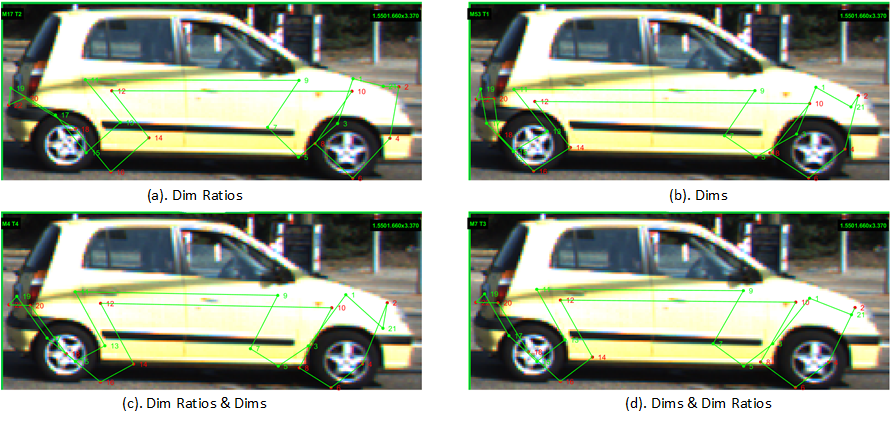
\includegraphics[width=1\textwidth]{model_selection_s.png}
	\caption[One labelled example of four model selection strategies.]{One labelled example of four model selection strategies. (a). Dim Ratios. (b). Dims. (c). Dim Ratios \& Dims. (d). Dims \& Dim Ratios. }
	\centering
	\label{figure:model_selection_s}
\end{figure}

\subsubsection{Difficulty Levels For Dataset Division}
KITTI set three levels for 3D object detection based on three factors: the height of the 2D bounding boxes, the degree of occlusion and truncation. In order to compare the influence brought by these three factors, we extend the division into nine levels, as shown in Table \ref{levels_d}. And Level 4 is used to evaluate other design choices because it is neither too complicated nor too simple.

\renewcommand{\arraystretch}{1.0}
\begin{table}[H]
	\centering
	\caption[Levels of difficulty.]{Levels of difficulty. Level 2, 6, and 8 corresponds to the Easy, Moderate, and Hard defined by KITTI \cite{Geiger2012CVPR}.}
	\label{levels_d}
	\resizebox{\textwidth}{!}{
	\begin{tabular}{|c|c|c|c|}
		\hline
		Difficulty level       & Min. bounding box height & Max. Occlusion   & Max. Occlusion \\ \hline
		Level 1   & 40 Px  & 0       & 0     \\ \hline
		\textbf{Level 2 (Easy)}     & \textbf{40 Px}  & \textbf{0}       & \textbf{15\%}  \\ \hline
		Level 3   & 40 Px  & 0, 1    & 15\%  \\ \hline
		Level 4   & 40 Px  & 0, 1    & 30\%  \\ \hline
		Level 5   & 32 Px  & 0, 1    & 30\%  \\ \hline
		\textbf{Level 6 (Moderate)} & \textbf{25 Px}  & \textbf{0, 1}    & \textbf{30\%}  \\ \hline
		Level 7   & 25 Px  & 0, 1, 2 & 30\%  \\ \hline
		\textbf{Level 8 (Hard)}     & \textbf{25 Px}  & \textbf{0, 1, 2} & \textbf{50\%}  \\ \hline
		Level 9   & 25 Px  & 0, 1, 2, 3       & 70\%  \\ \hline
	\end{tabular}
}
\end{table}

We train the network for these nine levels to their best with the identical foundation and the results of six tasks are shown in Table \ref{levels_p}. According to the performance of Level 1-3, we can conclude that our approach is robust to a slight degree of occlusion and truncation.  The performance of Level 3-5 shows that the size of vehicles in the image really affects the detection accuracy. Based on the decrease from Level 3 to Level 4 and Level 7 to Level 8, truncation also has a large negative impact on the detection accuracy. Compared with these two factors, occlusion has weaker influence in our approach. 

Besides, from the results we can see how error propagates in our approach. 3D bounding box estimation is a summation of the location, orientation, and dimension estimation tasks. Therefore, even if these three individual task has relatively good performance, their errors would propagate to and amplified the error of the ultimate task, 3D bounding box estimation.

% Please add the following required packages to your document preamble:
% \usepackage{graphicx}
\begin{table}[H]
	\centering
	\caption{Performance of six tasks at different difficult levels.}
	\label{levels_p}
	\resizebox{\textwidth}{!}{%
		\begin{tabular}{|c|c|c|c|c|c|c|}
			\hline
			& \begin{tabular}[c]{@{}c@{}}3D bounding\\ box estimation\end{tabular} & \begin{tabular}[c]{@{}c@{}}3D localization\\ ($Loc. < 1m$)\end{tabular} & \begin{tabular}[c]{@{}c@{}}3D orientation\\ estimation\end{tabular} & \begin{tabular}[c]{@{}c@{}}3D dimension\\ estimation\end{tabular} & \begin{tabular}[c]{@{}c@{}}2D part\\ localization\end{tabular} & \begin{tabular}[c]{@{}c@{}}2D part\\ visibility\end{tabular} \\ \hline
			Level 1 & 34.28 & 69.68 & \textbf{99.83} & 99.88 & \textbf{99.96} & \textbf{98.23} \\ \hline
			Level 2 & \textbf{35.56} & 70.73 & 99.66 & 99.88 & 99.77 & 98.16 \\ \hline
			Level 3 & 35.44 & \textbf{71.23} & 99.33 & \textbf{99.93} & 99.58 & 96.24 \\ \hline
			Level 4 & 32.97 & 69.22 & 99.34 & 99.73 & 99.25 & 95.97 \\ \hline
			Level 5 & 30.39 & 64.00 & 99.29 & 99.73 & 99.42 & 95.86 \\ \hline
			Level 6 & 28.20 & 56.31 & 99.39 & 99.87 & 99.52 & 95.85 \\ \hline
			Level 7 & 28.01 & 57.77 & 99.03 & 99.64 & 99.22 & 95.56 \\ \hline
			Level 8 & 25.79 & 57.68 & 98.60 & 99.81 & 98.82 & 95.37 \\ \hline
			Level 9 & 25.58 & 58.02 & 98.48 & 99.48 & 98.06 & 94.77 \\ \hline
		\end{tabular}%
	}
\end{table}

\subsubsection{Cost Function}

We have described the loss function we used in Section \ref{loss_functions} and here we give reasons for our choice.

The categorical cross entropy loss is the standard choice for multi-class classification but for regression, there are plenty of choices. We select out and do experiment on the following loss functions:  mean squared error \cite{4775883}, mean absolute error \cite{2005ClRes3079W}, Huber loss \cite{huber1964}, Charbonnier loss \cite{413553},  a robust smooth $L_1$ loss function defined in \cite{DBLP:journals/corr/Girshick15}, and our modified smooth $L_1$ loss function defined in Section \ref{loss_functions}.

We experiment with these loss functions with the same setup on Level 4 and evaluate their performance on six tasks with the validation data. The results are shown in Table \ref{p_loss_fcn}. Our modified loss for regression tasks (the first five) outperforms all the others and only has a slight impact on the classification task. The main reason for the modification is that we normalize the labels into the range $[1, 1]$ and most of them fall into the range $[-0.5, 0.5]$. 

\renewcommand{\arraystretch}{1.2}
\begin{table}[H]
	\centering
	\caption{Performance of six tasks with different loss functions.}
	\label{p_loss_fcn}
	\resizebox{\textwidth}{!}{
	\begin{tabular}{|c|c|c|c|c|c|c|}
		\hline
		Loss function & \begin{tabular}[c]{@{}c@{}}3D bounding\\ box estimation\end{tabular} & \begin{tabular}[c]{@{}c@{}}3D localization\\ ($Loc.<1m$)\end{tabular} & \begin{tabular}[c]{@{}c@{}}3D orientation\\ estimation\end{tabular} & \begin{tabular}[c]{@{}c@{}}3D dimension\\ estimation\end{tabular} & \begin{tabular}[c]{@{}c@{}}2D part \\ localization\end{tabular} & \begin{tabular}[c]{@{}c@{}}2D part\\ visibility\end{tabular} \\ \hline
		\begin{tabular}[c]{@{}c@{}}Charbonnier loss\\ $\epsilon$=0.01\end{tabular} & 28.94 & 58.57 & 98.30 & 99.59 & 98.09 & 93.95 \\ \hline
		\begin{tabular}[c]{@{}c@{}}Charbonnier loss\\ $\epsilon$=0.0001\end{tabular} & 27.3 & 59.04 & 97.89 & \textbf{99.73} & 97.7 & 92.27 \\ \hline
		\begin{tabular}[c]{@{}c@{}}Huber loss\\ $\delta$=0.5\end{tabular} & 25.87 & 58.77 & 98.42 & 99.59 & 98.06 & 94.54 \\ \hline
		mean absolute error & 4.3 & 17.54 & 90.02 & 92.42 & 86.59 & 93.24 \\ \hline
		mean squared error & 7.51 & 25.94 & 94.02 & 97.61 & 88.81 & 93.48 \\ \hline
		robust smooth $L_1$ & 26.21 & 61.09 & 98.47 & 99.66 & 98.11 & \textbf{94.66} \\ \hline
		modified smooth $L_1$ & \textbf{27.39} & \textbf{62.59} & \textbf{98.67} & \textbf{99.73} & \textbf{98.3} & 94.45 \\ \hline
	\end{tabular}%
}
\end{table}

Based on the experiment above, we tune the loss weights: $\lambda_{coord}$, $\lambda_{temp}$ and $\lambda_{visib}$, defined in Eq \ref{eq12}. As mentioned in Section \ref{normalization}, we have normalized the magnitude of all labels into the same range $[-1, 1]$. This label normalization alleviates the difficulties of loss weights tuning because we can focus on the importance of tasks without paying special attention to their quantities.


We apply grid search to find the optimal loss weight combination which results in best performance on the six tasks. Grid search is a common but sometimes expensive practice \cite{Goodfellow-et-al-2016} but the time to train our network is acceptable because we use pre-trained models to initialize our network. The $\lambda_{visib}$ is assigned 1, $\lambda_{coord}$ and $\lambda_{temp}$ are chosen from the set $\{1, 3, 10, 30\}$ because 2D coordinates and dimension proximity is much more important than visibility for 3D object detection. The results are shown in Table \ref{p_lw}. The $(\lambda_{coord}=10$, $\lambda_{temp}=1)$ combination is optimal among all choices \ie it performs better on four tasks and only slightly worse on the other two tasks than other weights combinations. This is because the 2D coordinates are used to perform 2D-3D matching and a small deviation of one point in the image can lead to a large difference in the world coordinate system. Besides, the dimension proximity cannot diverge too much due to the matching strategy where a big deviation only happens when all the predicted dimension ratios vectors are ridiculously wrong.


\renewcommand{\arraystretch}{1.2}
\begin{table}[H]
	\centering
	\caption{Performance of six tasks with different loss weights combinations.}
	\label{p_lw}
	\resizebox{\textwidth}{!}{%
		\begin{tabular}{|c|c|c|c|c|c|c|}
			\hline
			($\lambda_{coord}$, $\lambda_{temp}$) & \begin{tabular}[c]{@{}c@{}}3D bounding\\ box estimation\end{tabular} & \begin{tabular}[c]{@{}c@{}}3D localization\\ ($Loc.<1m$)\end{tabular} & \begin{tabular}[c]{@{}c@{}}3D orientation\\ estimation\end{tabular} & \begin{tabular}[c]{@{}c@{}}3D dimension\\ estimation\end{tabular} & \begin{tabular}[c]{@{}c@{}}2D part\\ localization\end{tabular} & \begin{tabular}[c]{@{}c@{}}2D part\\ visibility\end{tabular} \\ \hline
			(1, 1) & 29.35 & 63.89 & 98.53 & 99.66 & 98.39 & 94.98 \\ \hline
			(1, 3) & 25.19 & 56.93 & 97.87 & 99.59 & 97.7 & 94.18 \\ \hline
			(1, 10) & 24.71 & 53.65 & 98.05 & 99.66 & 97.61 & 94.41 \\ \hline
			(1, 30) & 19.59 & 45.39 & 97.68 & 99.59 & 96.46 & 93.92 \\ \hline
			(3, 1) & 29.28 & 61.84 & 98.78 & 99.59 & 98.56 & 94.71 \\ \hline
			(3, 3) & 29.76 & 63.89 & 98.63 & 99.66 & 98.55 & 94.72 \\ \hline
			(3, 10) & 25.67 & 58.7 & 98.04 & 99.52 & 97.56 & 94.28 \\ \hline
			(3, 30) & 21.98 & 49.69 & 98.32 & 99.59 & 97.18 & 93.99 \\ \hline
			(10, 1) & \textbf{34.06} & \textbf{68.46} & 99.16 & 99.66 & \textbf{98.98} & \textbf{95.18} \\ \hline
			(10, 3) & 30.58 & 63.41 & 98.71 & \textbf{99.73} & 98.61 & 94.38 \\ \hline
			(10, 10) & 32.7 & 66.28 & 98.60 & 99.59 & 98.62 & 94.52 \\ \hline
			(10, 30) & 27.03 & 60.27 & 98.09 & \textbf{99.73} & 97.79 & 93.96 \\ \hline
			(30, 1) & 33.17 & 66.96 & \textbf{99.24} & 99.66 & 98.95 & 94.91 \\ \hline
			(30, 3) & 31.4 & 66.62 & 98.87 & \textbf{99.73} & 98.88 & 94.43 \\ \hline
			(30, 10) & 31.74 & 68.12 & 98.69 & 99.66 & 98.61 & 94.46 \\ \hline
			(30, 30) & 31.19 & 65.32 & 98.66 & 99.52 & 98.36 & 93.43 \\ \hline
		\end{tabular}%
	}
\end{table}


\subsubsection{Learning Rate and Weight Decay}

Learning rate is one hyperparameter that determines how much the parameters of the network are updated with respect to the gradients of the cost function. It is perhaps the most crucial hyperparameter because it plays a more complicated and important role in affecting the effective capability of the model than the others. There is a typical U-shaped relationship between the learning rate and the model's performance. If it is too small, the training is more stable but the time to train the model is much longer and sometimes, the training might get stuck on a plateau region or around a saddle point. On the other hand, if it is too large, the training can converge more quickly but is more variable because it may fail to converge or even diverge. Only a proper learning rate can achieve the best performance of the model. Therefore, as Goodfellow \etal suggest that if you can only tune one hyperparameter, tune the learning rate \cite{Goodfellow-et-al-2016}.

Automatic learning rate selection methods alleviate the difficulty hugely, but they are too computational expensive so that we manually tune it. We first apply an ``LR range test" \cite{DBLP:journals/corr/Smith15a}, training the network for several epochs with the learning rate increasing linearly in a guessing range and then analysing the loss over these learning rates. From the test result in Figure \ref{figure:lr_test}, the proper learning rate falls in the range $[10^{-6}, 10^{-4}]$. 

\begin{figure}[H]		
	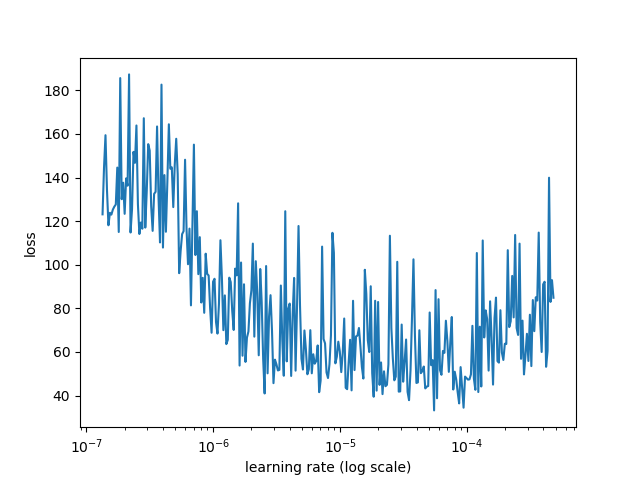
\includegraphics[width=0.8\textwidth]{LR_range_test.png}
	\caption[Results of ``LR range test".]{Results of ``LR range test": loss over monotonically increasing learning rate. }
	\centering
	\label{figure:lr_test}
\end{figure}

Weight decay is a regularization technique which is used to prevent the weights of the model getting too big as to be overfitting. Since Keras Optimizers \cite{chollet2015keras} take both learning rate and weight decay as input parameters, we apply grid search for both of them together. The results are shown in Table \ref{lrd}. The combination of $(10^{-5}, 10^{-6})$ for learning rate and weight decay respectively achieves the best performance except for 2D part visibility classification with $0.2\%$ lower. Therefore, we select this combination. The best results in Table \ref{lrd} is worse than those in Table \ref{p_lw} because we set all loss weights as 1 here. 

% Please add the following required packages to your document preamble:
% \usepackage{graphicx}
\begin{table}[H]
	\centering
	\caption{Performance of six tasks with different learning rate and weight decay combinations}
	\label{lrd}
	\resizebox{\textwidth}{!}{%
		\begin{tabular}{|c|c|c|c|c|c|c|}
			\hline
			\begin{tabular}[c]{@{}c@{}}(learning rate, \\weight decay)\end{tabular} & \begin{tabular}[c]{@{}c@{}}3D bounding\\ box estimation\end{tabular} & \begin{tabular}[c]{@{}c@{}}3D localization\\ ($Loc.<1m$)\end{tabular} & \begin{tabular}[c]{@{}c@{}}3D orientation\\ estimation\end{tabular} & \begin{tabular}[c]{@{}c@{}}3D dimension\\ estimation\end{tabular} & \begin{tabular}[c]{@{}c@{}}2D part\\ localization\end{tabular} & \begin{tabular}[c]{@{}c@{}}2D part\\ visibility\end{tabular} \\ \hline
			$(10^{-4}, 10^{-4})$ & 25.05 & 56.38 & 97.65 & 99.66 & 98.15 & 94.84 \\ \hline
			$(10^{-4}, 10^{-5})$ & 29.15 & 60.82 & 97.96 & 99.59 & 98.25 & 95.08 \\ \hline
			$(10^{-4}, 10^{-6})$ & 26.69 & 56.59 & 97.80 & \textbf{99.73} & 98.38 & \textbf{95.09} \\ \hline
			$(10^{-4}, 10^{-7})$ & 27.85 & 59.45 & 97.94 & \textbf{99.73} & 98.22 & 94.97 \\ \hline
			$(10^{-5}, 10^{-4})$ & 26.96 & 59.59 & 97.90 & 99.39 & 97.51 & 93.17 \\ \hline
			$(10^{-5}, 10^{-5})$ & 30.95 & 62.46 & 98.52 & 99.52 & 98.09 & 94.1 \\ \hline
			$(10^{-5}, 10^{-6})$ & \textbf{32.06} & \textbf{63.07} & \textbf{98.62} & \textbf{99.73} & \textbf{98.56} & 94.87 \\ \hline
			$(10^{-5}, 10^{-7})$ & 27.1 & 62.66 & 98.44 & \textbf{99.73} & 98.27 & 94.55 \\ \hline
			$(10^{-6}, 10^{-4})$ & 18.16 & 44.23 & 96.15 & 99.04 & 95.1 & 89.17 \\ \hline
			$(10^{-6}, 10^{-5})$ & 19.52 & 47.92 & 97.08 & 99.04 & 95.77 & 90.48 \\ \hline
			$(10^{-6}, 10^{-6})$ & 17.82 & 46.01 & 96.85 & 98.84 & 95.18 & 89.71 \\ \hline
			$(10^{-6}, 10^{-7})$ & 17.2 & 47.44 & 96.87 & 98.98 & 95.53 & 90.08 \\ \hline
		\end{tabular}%
	}
\end{table}

\subsubsection{Feature Extractor}
Our baseline network uses ResNet50 as feature extractor. But there are several other out-of-shelf networks with pre-trained weights so that we carry out experiments on them. The other base nets we choose are VGG16, VGG19 \cite{DBLP:SimonyanZ14a}, InceptionV3 \cite{DBLP:journals/corr/SzegedyVISW15}, Xception \cite{DBLP:journals/corr/Chollet16a}, DenseNet121, DenseNet169, DenseNet201\cite{DBLP:journals/corr/HuangLW16a}.

As before, we train all the models with different base nets on the same setup on data Level 4. Their performance on six tasks are shown in Table \ref{basenets}. According to their performance, only VGG19 can perform better than ResNet50 overall. Therefore, we include VGG19 for our final evaluation in Section \ref{exp_res}.

\begin{table}[H]
	\centering
	\caption{Performance of six tasks with different base nets.}
	\label{basenets}
	\resizebox{\textwidth}{!}{%
		\begin{tabular}{|c|c|c|c|c|c|c|}
			\hline
			Base Net & \begin{tabular}[c]{@{}c@{}}3D bounding\\ box estimation\end{tabular} & \begin{tabular}[c]{@{}c@{}}3D localization\\ ($Loc.<1m$)\end{tabular} & \begin{tabular}[c]{@{}c@{}}3D orientation\\ estimation\end{tabular} & \begin{tabular}[c]{@{}c@{}}3D dimension\\ estimation\end{tabular} & \begin{tabular}[c]{@{}c@{}}2D part\\ localization\end{tabular} & \begin{tabular}[c]{@{}c@{}}2D part\\ visibility\end{tabular} \\ \hline
			ResNet50 & \textbf{30.85} & \textbf{64.98} & \textbf{99.03} & 99.73 & \textbf{98.77} & 94.74 \\ \hline
			VGG16 & 29.22 & 57.82 & 98.54 & \textbf{99.86} & 98.44 & \textbf{95.76} \\ \hline
			VGG19 & \textbf{31.54} & 64.23 & \textbf{99.22} & \textbf{99.93} & \textbf{98.68} & \textbf{96.05} \\ \hline
			InceptionV3 & 27.51 & 63.07 & 97.90 & 99.25 & 97.82 & 93.83 \\ \hline
			Xception & 21.09 & 49.83 & 96.05 & 98.91 & 95.22 & 89.17 \\ \hline
			DenseNet121 & 26.28 & 59.73 & 98.15 & 99.52 & 97.47 & 93.26 \\ \hline
			DenseNet169 & 30.24 & \textbf{65.05} & 98.27 & 99.59 & 98.05 & 93.8 \\ \hline
			DenseNet201 & 27.3 & 61.37 & 98.69 & 99.59 & 98.08 & 93.45 \\ \hline
		\end{tabular}%
	}
\end{table}

\subsubsection{Selection of Characteristic Points}

The number of characteristic points is another factor that influences the performance. Theoretically, the more points the better accuracy of 2D-3D matching because it is more robust to outliers. The outliers are eliminated via RANSAC \cite{Fischler:1981:RSC:358669.358692} during the 2D-3D matching. But the labelling of these points is time-consuming and demanding. Moreover, the exact locations of points also affect the performance. Some points may be hard to detect correctly with the network due to their context in the image and some even distribute differently among various shapes of vehicles. 

\begin{figure}[ht]		
	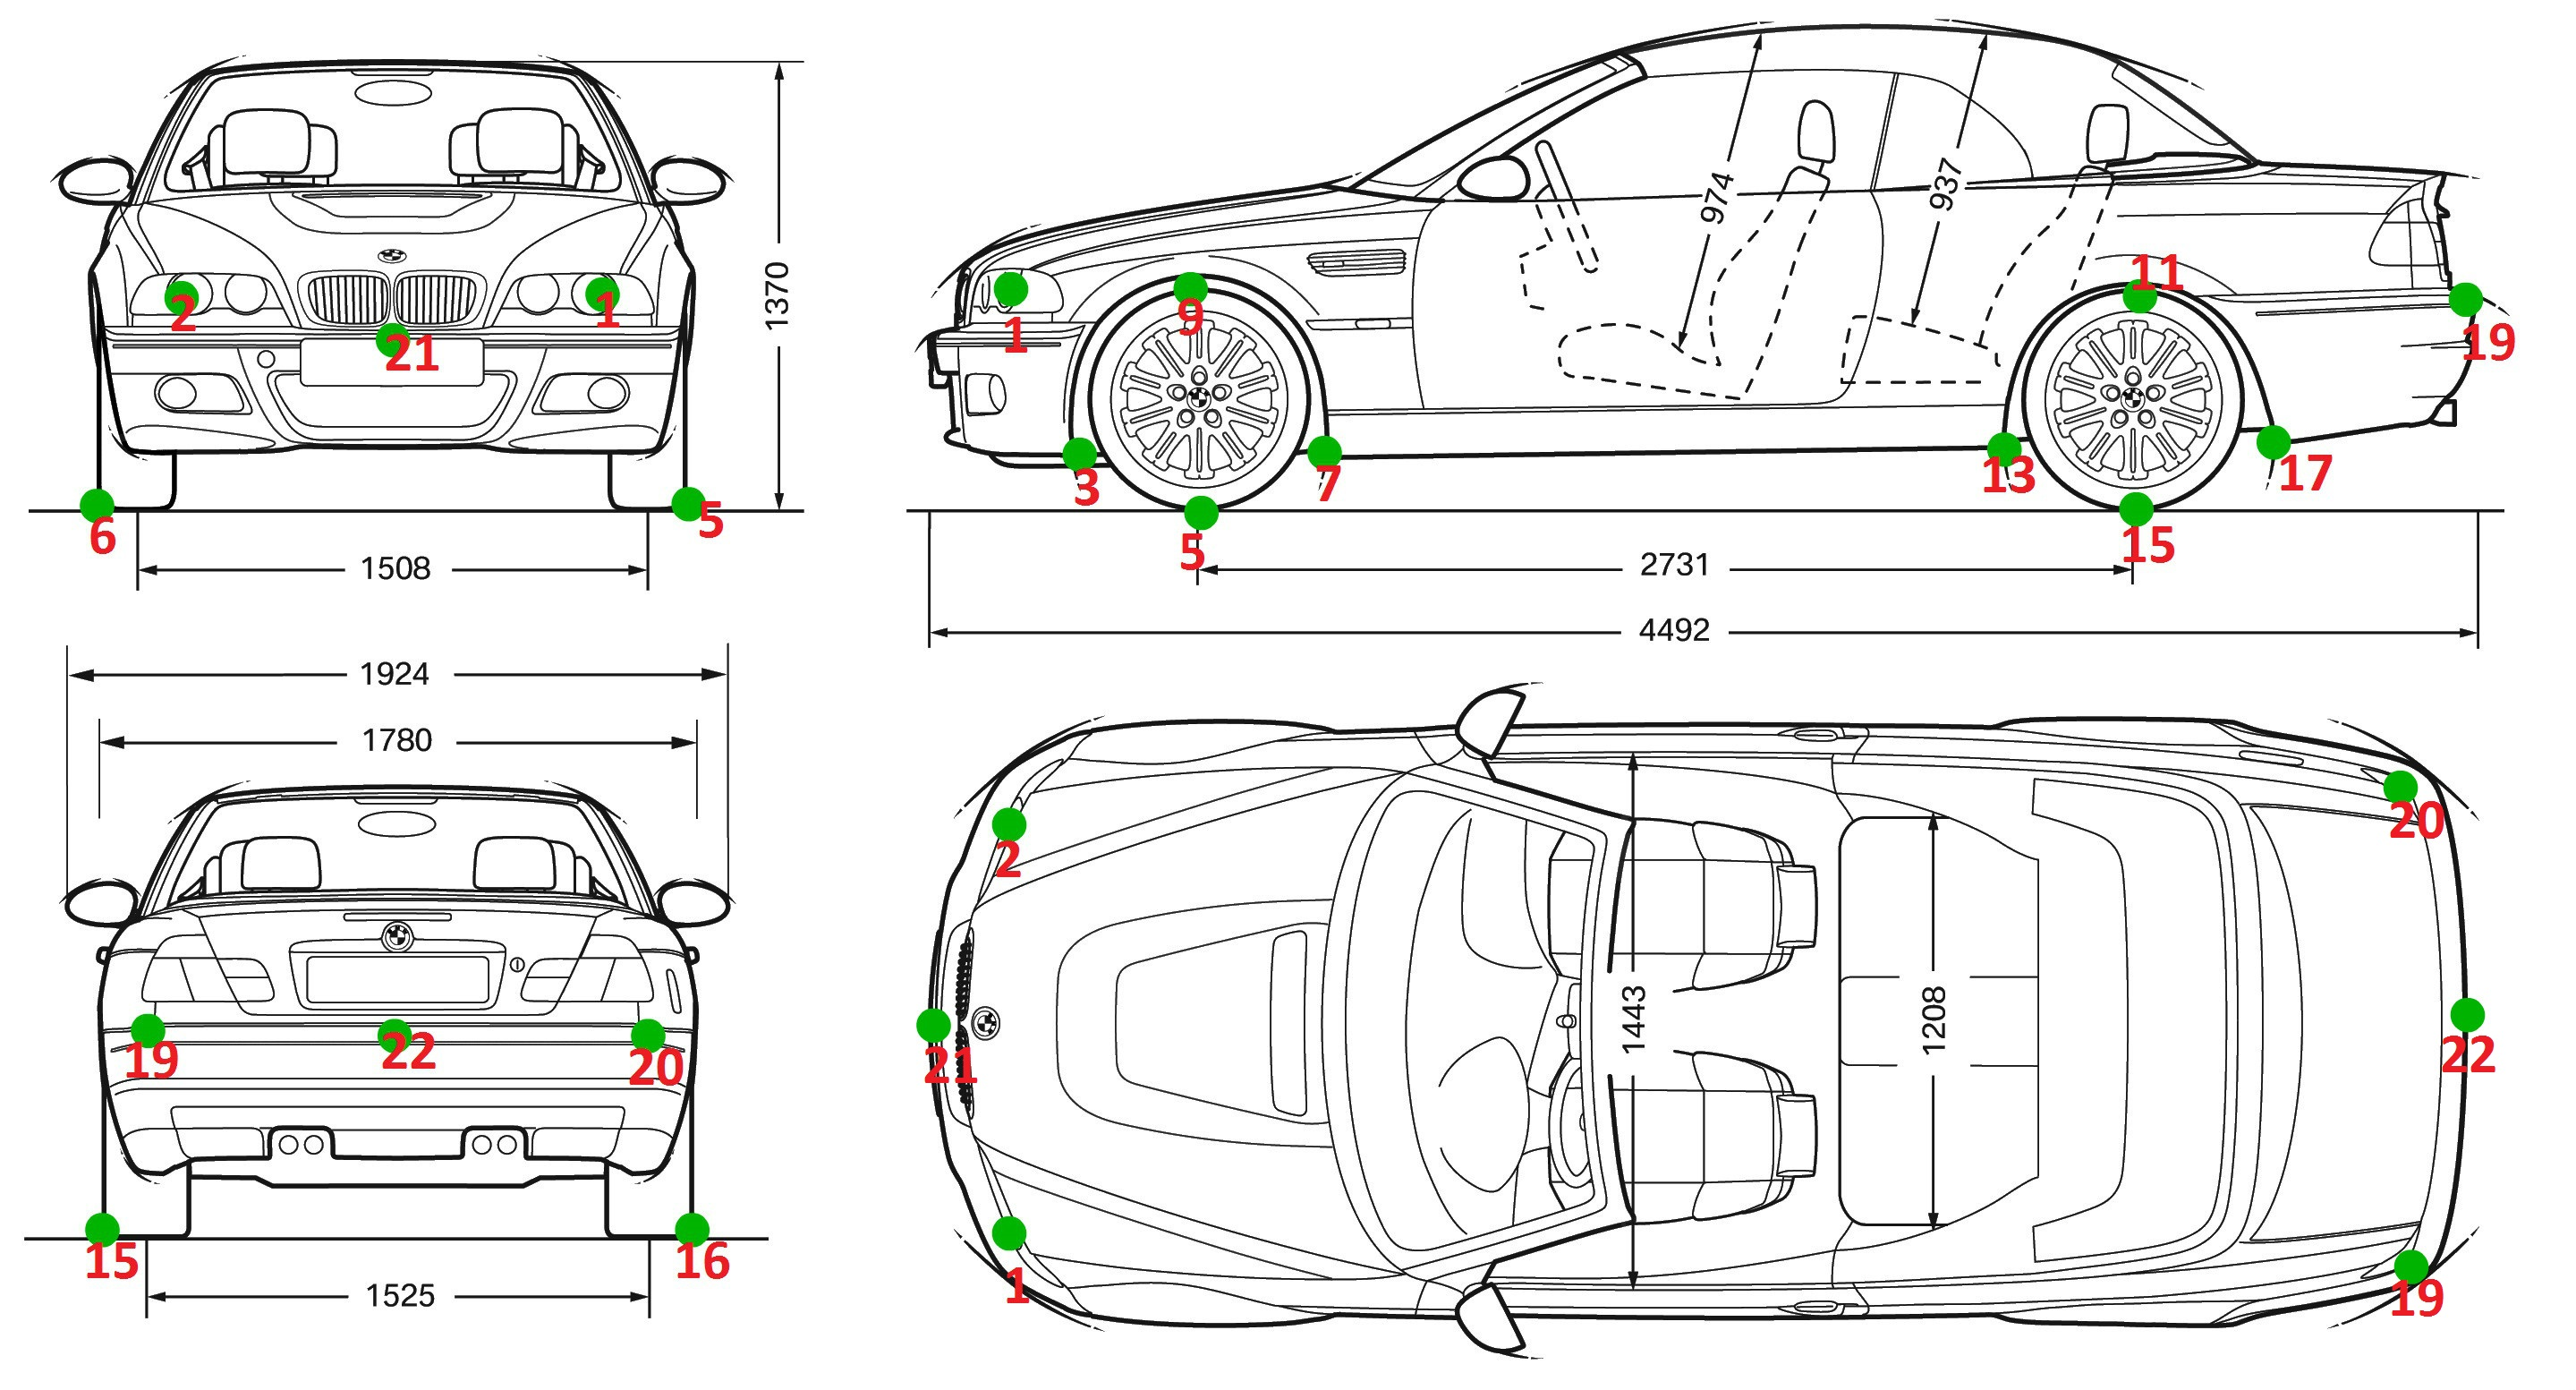
\includegraphics[width=1\textwidth]{point_notation_22.jpg}
	\caption[The schematic diagram of 22 characteristic points.]{The schematic diagram of 22 characteristic points. point 1 and 2 denotes the centre of two headlights; point 3-18 are around four wheels; point 19 and 20 denote two rear corners; and point 21 and 22 denotes the frontmost and  backmost points along the ordinate axis of the vehicle.}
	\centering
	\label{figure:point_notation_22}
\end{figure}

As the Figure \ref{figure:point_notation_22} shows, we initially label 22 points for each model to construct its corresponding 3D sketch. The points around four wheels are most important because their geometric characters are most stable and rigid, and usually, half of them are visible if not occluded by other objects. However, points 1, 2, 19, and 20 around the front and rear may vary a lot w.r.t. different shapes of the vehicles. We still consider them because they have clear semantic meaning and we may need these points when the points around wheels are not visible, \eg when the vehicle is following the target vehicle on the straight lane. The geometric property of point 21 and 22 are stable but their context is not as clear as the points around the wheels.

Therefore, we do some experiment on the selection of these points. We select three cases: 1). 16 points: points 3-18; 2). 20 points: points 1-18 and points 21-22; 3). 22 points: point 1-22. We train these three case on data Level 1-9 to compare their influence thoroughly. The reason for training on nine levels instead of only Level 4 as before is that the size of the 2D bounding box and degree of the occlusion and truncation impact the geometric appearance of vehicles in the images and thus affect the detection of these points. The experiment results are shown in Table \ref{point_selection}.  According to the results, the 22-point case works best or just slightly worse, which justifies our guess. And a surprising phenomenon is that 16-point case performs worst on most Levels. The reason might be that there is at most only one face can be visible in 16-point case due to the occlusion and truncation and there is only a small portion, one quarter, of fully visible cars in KITTI dataset.

%when the input patch is relatively bigger, \ie the minimal height for a 2D bounding box is 40 pixels. This is because when the vehicles are large in the image, it is easier to estimate the 2D coordinates and the dimension proximity and in this scenario, the more the points, the better the performance. However, when very small vehicles are taken into consideration, it becomes harder to predict the 2D coordinates correctly because these key points in a small vehicle locate very close to each other. 


% 9 levels
\begin{table}[H]
	\centering
	\caption{Performance of six tasks with different data difficulty level and different point selection cases.}
	\label{my-label}
	\resizebox{\textwidth}{!}{%
		\begin{tabular}{|c|c|c|c|c|c|c|c|}
			\hline
			Level & \#points & \begin{tabular}[c]{@{}c@{}}3D bounding\\ box estimation\end{tabular} & \begin{tabular}[c]{@{}c@{}}3D localization\\ ($Loc.<1m$)\end{tabular} & \begin{tabular}[c]{@{}c@{}}3D orientation\\ estimation\end{tabular} & \begin{tabular}[c]{@{}c@{}}3D dimension\\ estimation\end{tabular} & \begin{tabular}[c]{@{}c@{}}2D part\\ localization\end{tabular} & \begin{tabular}[c]{@{}c@{}}2D part\\ visibility\end{tabular} \\ \hline
			\multirow{3}{*}{Level 1} & P16 & 32.43 & 65.1 & 99.74 & \textbf{99.88} & 99.71 & 97.73 \\ \cline{2-8} 
			& P20 & 33.54 & 65.97 & \textbf{99.77} & 99.63 & \textbf{99.78} & 98.03 \\ \cline{2-8} 
			& P22 & \textbf{35.27} & \textbf{68.94} & 99.72 & \textbf{99.88} & 99.77 & \textbf{98.04} \\ \hline
			\multicolumn{8}{|c|}{} \\ \hline
			\multirow{3}{*}{Level 2} & P16 & 31.28 & 64.81 & 99.75 & \textbf{99.88} & \textbf{99.48} & \textbf{97.82} \\ \cline{2-8} 
			& P20 & 34 & 67.77 & \textbf{99.76} & 99.76 & 99.32 & 97.77 \\ \cline{2-8} 
			& P22 & \textbf{34.83} & \textbf{69.43} & 99.16 & 99.76 & 99.35 & 97.73 \\ \hline
			\multicolumn{8}{|c|}{} \\ \hline
			\multirow{3}{*}{Level 3} & P16 & 30.84 & 64.02 & 98.95 & \textbf{99.84} & 98.96 & 95.21 \\ \cline{2-8} 
			& P20 & \textbf{32.49} & \textbf{66.81} & 98.96 & 99.79 & 98.91 & \textbf{95.5} \\ \cline{2-8} 
			& P22 & 31.89 & 61.93 & \textbf{99.1} & 99.92 & \textbf{99.37} & 95.03 \\ \hline
			\multicolumn{8}{|c|}{} \\ \hline
			\multirow{3}{*}{Level 4} & P16 & 29.69 & 62.12 & 98.99 & 99.66 & 98.87 & 94.45 \\ \cline{2-8} 
			& P20 & 30.92 & 65.6 & \textbf{99.01} & \textbf{99.73} & 98.72 & 94.65 \\ \cline{2-8} 
			& P22 & \textbf{31.47} & \textbf{66.48} & 98.86 & \textbf{99.73} & \textbf{98.94} & \textbf{94.96} \\ \hline
			\multicolumn{8}{|c|}{} \\ \hline
			\multirow{3}{*}{Level 5} & P16 & 28.1 & 58.61 & \textbf{99.09} & \textbf{99.78} & \textbf{98.99} & \textbf{94.87} \\ \cline{2-8} 
			& P20 & \textbf{29.41} & 59.91 & 98.67 & 99.73 & 98.65 & 94.53 \\ \cline{2-8} 
			& P22 & 28.98 & \textbf{60.89} & 98.68 & 99.62 & \textbf{98.99} & 94.01 \\ \hline
			\multicolumn{8}{|c|}{} \\ \hline
			\multirow{3}{*}{Level 6} & P16 & 25.39 & 56.22 & \textbf{99.05} & \textbf{99.64} & 98.88 & 94.98 \\ \cline{2-8} 
			& P20 & 26.68 & 57.16 & 98.55 & 99.6 & \textbf{98.9} & 94.92 \\ \cline{2-8} 
			& P22 & \textbf{28.16} & \textbf{57.21} & 98.86 & \textbf{99.64} & 98.89 & \textbf{95.02} \\ \hline
			\multicolumn{8}{|c|}{} \\ \hline
			\multirow{3}{*}{Level 7} & P16 & 23.7 & 53.1 & \textbf{98.81} & 99.6 & \textbf{98.61} & 93.87 \\ \cline{2-8} 
			& P20 & 24.1 & 52.7 & 97.83 & 99.54 & 98.48 & \textbf{94.24} \\ \cline{2-8} 
			& P22 & \textbf{24.73} & \textbf{55.55} & 98.03 & \textbf{99.7} & 98.46 & 94.02 \\ \hline
			\multicolumn{8}{|c|}{} \\ \hline
			\multirow{3}{*}{Level 8} & P16 & 24.04 & 53.39 & \textbf{98.53} & \textbf{99.55} & \textbf{98.28} & \textbf{94.15} \\ \cline{2-8} 
			& P20 & 22.86 & 51.35 & 97.30 & 99.48 & 97.52 & 93.92 \\ \cline{2-8} 
			& P22 & \textbf{24.26} & \textbf{53.56} & 97.5 & 99.48 & 97.8 & 93.45 \\ \hline
			\multicolumn{8}{|c|}{} \\ \hline
			\multirow{3}{*}{Level 9} & P16 & 22.51 & 50.46 & \textbf{97.48} & 99.24 & 96.89 & 93.16 \\ \cline{2-8} 
			& P20 & 20.05 & 47.75 & 96.78 & 99.21 & 96.05 & 92.59 \\ \cline{2-8} 
			& P22 & \textbf{24.27} & \textbf{52.86} & 97.13 & \textbf{99.3} & \textbf{96.94} & \textbf{93.44} \\ \hline
		\end{tabular}%
	}
\end{table}
\clearpage


\subsection{Experiment Results}
\label{exp_res}
In this subsection, we present the best results of six tasks achieved by our approach and compare them with the state-of-the-art works on 3D vehicle detection.

\subsubsection{3D Bounding Box Estimation} 
3D vehicle detection refers to the 3D bounding box estimation of the target vehicles in the images. A 3D bounding box is estimated correctly, if $IoU>0.7$. Our approach is based on 2D object detection, so in order to be comparable with other methods, we eliminate the influence of this foundation by multiplying our results with the top accuracy of 2D car detection in KITTI achieved by iDST-VC \cite{2dobject}. Our results and the comparison are shown in Table \ref{3D_vehicle_detection}. A LiDAR-based method, VoxelNet++ \cite{DBLP:journals/corr/abs-1711-06396}, achieves the best performance currently. Based on the assumption above, our method currently ranks at the middle ($24^{th}$) on 3D vehicle detection benchmark \cite{3dobject}. It can achieve similar performance as VoxelNet basic \cite{DBLP:journals/corr/abs-1711-06396}. It outperforms all traceable image-based methods and some of the LiDAR-based methods. For more comparison, check \cite{3dobject}. Besides, our method performs 3D detection for all cars and vans on KITTI dataset while the results from other methods are for cars only. Therefore, theoretically, the performance of our approach on cars is at least not worse than on both cars and vans. 


\begin{table}[H]
	\centering
	\caption[Comparison of the 3D bounding box estimation performance.]{Comparison of the 3D bounding box estimation on official KITTI dataset for cars (ours is for cars and vans)}
	\label{3D_vehicle_detection}
	\begin{tabular}{|c|c|c|c|c|}
		\hline
		Method                                                                   & Type  & Easy           & Moderate       & Hard           \\ \hline
		3D-SSMFCNN \cite{novakmaster2017}                       & Mono  & 2.39           & 2.28           & 1.52           \\ \hline
		A3DODWTDA \cite{erino397fregu856master2018}             & Mono  & 6.76           & 6.45           & 4.87           \\ \hline
		DoBEM \cite{8088147}                                    & LiDAR & 7.42           & 6.95           & 13.45          \\ \hline
		LMNetV2 \cite{2018arXiv180504902M}                      & LiDAR & 14.75          & 15.24          & 12.85          \\ \hline
		VoxelNet basic \cite{DBLP:journals/corr/abs-1711-06396} & LiDAR & 29.70          & 24.35          & 23.52          \\ \hline
		VoxelNet++ \cite{DBLP:journals/corr/abs-1711-06396}     & LiDAR & \textbf{83.13} & \textbf{73.66} & \textbf{66.20} \\ \hline
		Ours (ResNet50)                                                          & Mono  & 30.90          & 24.16          & 18.53          \\ \hline
		Ours (VGG19)																& Mono	& 30.36	& 23.92	& 20.11 \\ \hline
		
	\end{tabular}
\end{table}


\subsubsection{3D Localization}
3D localization refers to the estimation of the location of the vehicle's centre. We follow the evaluation metric used by \cite{DBLP:journals/corr/MousavianAFK16, DBLP:journals/corr/ChabotCRTC17} that a 3D localization is correct if the distance between the true and predicted centre is smaller than a threshold and 1 meter and 2 meters are used as thresholds. And we borrow the idea from \cite{DBLP:journals/corr/MousavianAFK16} to calculate the 3D Localization accuracy, which is the ratio between Average Localization Precision (ALP) and Average Precision (AP), for other methods. We present our results and the comparison in Table \ref{3d_local}. Clearly, our method outperforms all other monocular methods, while cannot match the performance against the stereo 3DOP \cite{Chen:2015:OPA:2969239.2969287}.


\begin{table}[H]
	\centering
	\caption[Comparison of the 3D localization performance.]{Comparison of the 3D localization accuracy on official KITTI dataset for cars (ours is for cars and vans).}
	\label{3d_local}
	\resizebox{\textwidth}{!}{%
		\begin{tabular}{|c|c|c|c|c|c|c|c|}
			\hline
			\multirow{2}{*}{Method}                                      & \multirow{2}{*}{Type} & \multicolumn{3}{c|}{Loc. \textless 1m}           & \multicolumn{3}{c|}{Loc. \textless 2m}           \\ \cline{3-8} 
			&                       & Easy           & Moderate       & Hard           & Easy           & Moderate       & Hard           \\ \hline
			3DOP \cite{Chen:2015:OPA:2969239.2969287}   & Stereo                & \textbf{83.69} & \textbf{65.96} & \textbf{65.71} & \textbf{98.57} & \textbf{88.08} & \textbf{91.56} \\ \hline
			DPM \cite{5255236}                          & Mono                  & 34.33          & 29.02          & 29.18          & 56.48          & 46.69          & 46.17          \\ \hline
			3DVP \cite{xiang2015data}                   & Mono                  & 52.15          & 45.24          & 42.40          & 76.10          & 68.00          & 64.84          \\ \hline
			SubCNN \cite{DBLP:journals/corr/XiangCLS16} & Mono                  & 43.26          & 34.86          & 32.75          & 77.66          & 63.12          & 59.33          \\ \hline
			Ours (ResNet50)                                              & Mono                  & 67.87          & 59.96          & 51.38          & 87.56                & 79.83                & 73.11                \\ \hline
			Ours (VGG19)	                                             & Mono	                  & 68.25	          & 56.58	          & 54.53		          & 88.39	          & 78.63	          & 77.49                 \\ \hline
			
		\end{tabular}%
	}
\end{table}

\subsubsection{3D Orientation Estimation}
3D Orientation Estimation refers to the estimation of rotation of vehicle along the Y-axis (yaw axis), $r_y$, in the camera coordinate systems. The evaluation metric is Orientation Score (OS), which is the ratio between Average Orientation Estimation (AOS) and Average Precision (AP) \cite{DBLP:journals/corr/MousavianAFK16}. Table \ref{os_cmp} shows the results of our methods and other state-of-the-art ones. According to the statistics, our method achieves the start-of-the-art level performance for 3D orientation estimation. The VGG19 version even achieves the best performance on Easy level.


\begin{table}[H]
	\centering
	\caption[Comparison of the 3D orientation estimation performance.]{Comparison of the Orientation Score (OS) on official KITTI dataset for cars (ours is for cars and vans).}
	\label{os_cmp}
\begin{tabular}{|c|c|c|c|c|}
	\hline
	Method                                                                        & Type   & Easy           & Moderate       & Hard           \\ \hline
	3DOP \cite{Chen:2015:OPA:2969239.2969287}                    & Stereo & 98.28          & 97.13          & 96.73          \\ \hline
	Mono3D \cite{cvpr16chen}                                     & Mono   & 98.57          & 97.69          & 97.31          \\ \hline
	SubCNN \cite{DBLP:journals/corr/XiangCLS16}                  & Mono   & 99.84          & 99.52          & 99.25          \\ \hline
	Deep3DBox \cite{DBLP:journals/corr/MousavianAFK16}           & Mono   & 99.91 & 99.67          & 99.46          \\ \hline
	DeepMANTA (GoogLeNet) \cite{DBLP:journals/corr/ChabotCRTC17} & Mono   & 99.85          & \textbf{99.75} & \textbf{99.55} \\ \hline
	DeepMANTA (VGG16) \cite{DBLP:journals/corr/ChabotCRTC17}     & Mono   & 99.88          & 99.69          & 99.49          \\ \hline
	Ours (ResNet50)                                                               & Mono   & 99.88          & 98.78          & 97.39          \\ \hline
	Ours (VGG19)																	& Mono	 & \textbf{99.94}	       & 99.09	      & 98.43         \\ \hline
	
\end{tabular}
\end{table}

\subsubsection{3D dimension estimation, 2D part localization, and 2D part visibility}
Our approach is developed based on DeepMANTA \cite{DBLP:journals/corr/ChabotCRTC17}, so only DeepMANTA shares these three tasks with us. We present the results of DeepMANTA and our approach in Table \ref{the_rest_3}. And ours outperforms DeepMANTA on all these three tasks at all difficulty levels.

\begin{table}[H]
	\centering
	\caption[Comparison of the performance of 3D dimension estimation, 2D part localization, and 2D part visibility.]{Comparison of 3D dimension estimation, 2D part localization, and 2D part visibility on official KITTI dataset for cars (ours is for cars and vans).}
	\label{the_rest_3}
	\resizebox{\textwidth}{!}{%
		\begin{tabular}{|c|c|c|c|c|c|c|c|c|c|c|}
			\hline
			\multirow{2}{*}{Method} & \multirow{2}{*}{Type} & \multicolumn{3}{c|}{3D dimension estimation} & \multicolumn{3}{c|}{2D part localization} & \multicolumn{3}{c|}{2D part visibility} \\ \cline{3-11} 
			&  & Easy & Moderate & Hard & Easy & Moderate & Hard & Easy & Moderate & Hard \\ \hline
			DeepMANTA \cite{DBLP:journals/corr/ChabotCRTC17} & Mono & 97.54 & 90.79 & 82.64 & 92.48 & 85.08 & 76.9 & 94.04 & 86.62 & 78.72 \\ \hline
			Ours (ResNet50) & Mono & 99.76 & 99.6 & 99.48 & 99.32 & 98.9 & 97.52 & 97.77 & 94.92 & 93.92 \\ \hline
			Ours (VGG19) & Mono & \textbf{100} & \textbf{99.78} & \textbf{99.77} & \textbf{99.96} & \textbf{99.21} & \textbf{98.4} & \textbf{98.36} & \textbf{96.06} & \textbf{95.52} \\ \hline
		\end{tabular}
	}
\end{table}


\clearpage


\section{Discussion}
\label{discussion}

In this section, we discuss the deficiencies of our approach, analyse their causes and propose some possible improvements.

\subsection{Deficiency of 2D Coordinate Labelling}
\label{2d_def}
\subsubsection{Deficiency of Our Labelling Approach}
Our approach requires accurate 2D coordinates of characteristic points to perform 2D-3D matching to calculate the location and orientation of the vehicles. However, precisely labelling these points is demanding and even impossible for some vehicles with our semi-automatic labelling tool. The deficiency of labelling results from our labelling approach and the KITTI dataset.

Due to the variety of dimensions and shapes of vehicles, it is very hard to find a model that exactly matches the target vehicle with a small set of models. But if we expand the model set to cover all vehicles, the required quantity is too huge to satisfy. Therefore, we can only use a small set of models which means that the approximation and scaling are inevitable. And this will introduce errors to the labelling of 2D coordinates. Figure \ref{figure:label_def} (a) and (b) show two bad labelled examples. The imprecision of (a) results from the approximation of model matching, \ie most points are labelled correctly but point 1-6 are not. This is because the model can't perfectly fit the vehicle. The wrongly labelled points around wheels in Figure \ref{figure:label_def} (b) results from the scaling the model to fit the vehicle so that, for example, the distance between point 4 and 8 are larger than the diameter of the wheel. The other pairs of points around the wheel have the similar situation so that most points are not labelled correctly for this vehicle.

\subsubsection{Deficiency of KITTI Dataset Labelling}
Our labelling approach requires accurate labels of the dataset because 2D points are very sensitive to the exact location of the target vehicle. But some of the KITTI images are not labelled so well that our approach makes mistakes. There are three main deficiencies of the KITTI labelling as shown in Figure \ref{figure:label_def} (f), (g), and (h). (f) shows the 3D bounding box ground truth of this vehicle is not correctly labelled. The 3D bounding box does not encompass the vehicle, especially the rear part, which leads to wrong labelling. (g) and (h) shows that our approach wrong labels the 2D points due to the assumption of KITTI that the vehicle only rotates along the yaw axis rather than the roll and pitch axis.

\begin{figure}[H]		
	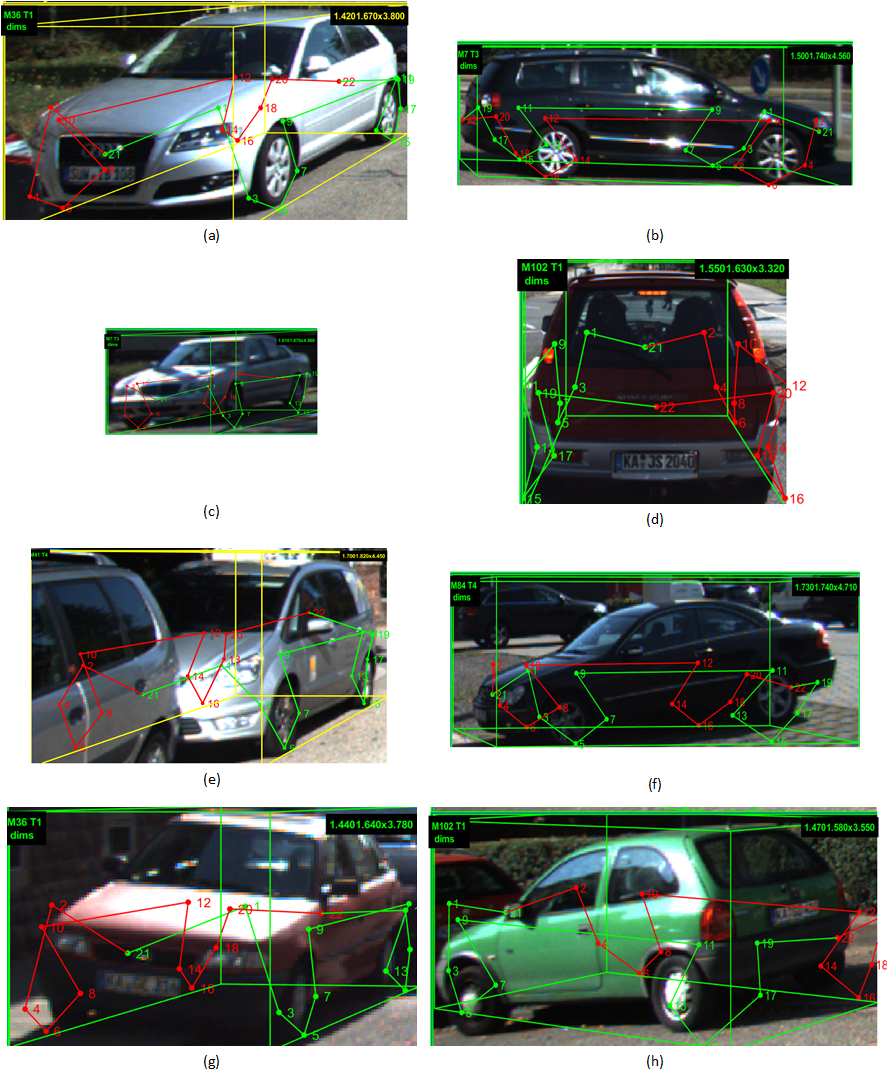
\includegraphics[width=0.8\textwidth]{label_def.png}
	\caption[Labelling examples of 2D points with the original size.]{Labelling examples with the original vehicle size. (a). Approximation results in inaccurate labels for point 1-6. (b). Scaling leads to bad labelling for points around the wheels. (c). One of the very small vehicles is able to be labelled with our approach. (d). The example that the side faces are not visible is can be labelled with our approach. (e). The occluded vehicle can also be labelled with our approach. (f). The 3D bounding box ground truth of this vehicle is not correctly labelled in KITTI dataset. (g). KITTI does not consider the rotation along the roll axis, which results in bad labelling. (h). KITTI does not consider the rotation along the pitch axis, which results in totally wrong labelling.}
	\centering
	\label{figure:label_def}
\end{figure}

\subsubsection{Possible Improvements}
Despite the drawbacks of our labelling approach, it still has some advantages. Our approach can label very small vehicles in the image as shown in Figure \ref{figure:label_def} (c). Besides, it can label the self-occluded points as in Figure \ref{figure:label_def} (d) and the occluded and truncated points in Figure \ref{figure:label_def} (e). 

Therefore, if labelling labour is allowed, we can manually label the visible points for big vehicles and use the projection property and the geometry constraints to automatically generate the the labels for corresponding points. Therefore, we have more accurate points for big vehicles. And for small and highly occluded or truncated vehicles, it is suitable to use our approach to label them. Because manually labelling these special vehicles is almost impossible and the error of our labelling approach can be decreased due to the quantities.


\subsection{Deficiency of Visibility Labelling}
\subsubsection{Deficiency of Our Labelling Approach}
As described in Section \ref{visibility}, we label the visibility property of characteristic points with the help of the rotation $r_y$, other labelled objects, and the size of images. But there are two main shortcomings. The first one is that the 2D bounding box of a vehicle is larger in the image than its real shape which makes our approach mistake the visible or self-occlude points as occluded. Figure \ref{figure:visib_def} (a). shows an example of labelling the self-occluded points as occluded, which leads to wrong labels. Another shortcoming is that our approach can't take the unlabelled objects into consideration so that it automatically ignores them during labelling. Figure \ref{figure:visib_def} (b) and (c) show two examples for this case. Our approach cannot consider the traffic sign in (b) and the building in (c) and thus, it fails to label these occluded points correctly.


\begin{figure}[H]		
	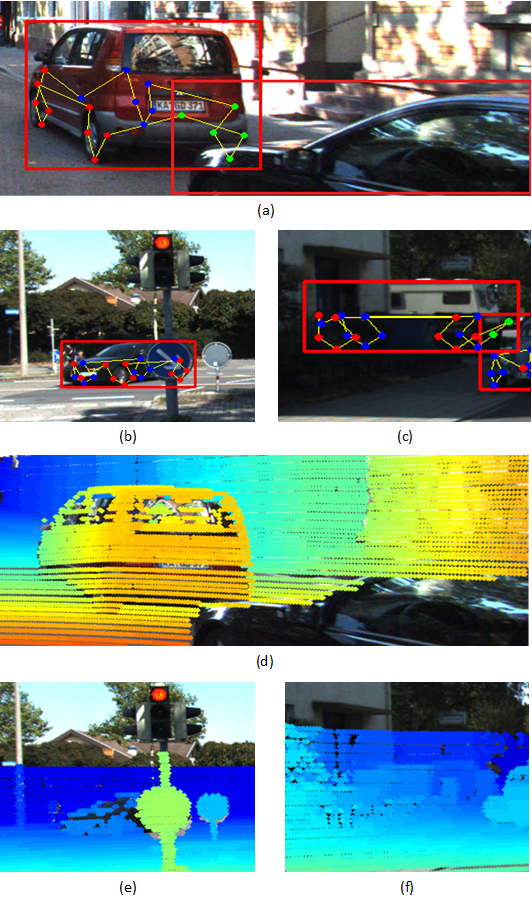
\includegraphics[width=0.7\textwidth]{visib_def.png}
	\caption[Labelling examples for visibility with the original size.]{Labelling examples for visibility with the original size. (a). The 2D bounding box is larger than the vehicle's real size, which results in labelling the self-occluded points as occluded. (b). KITTI doesn't label the traffic sign so that our approach can't label the occluded points correctly. (c). KITTI doesn't label the building so that our approach can't label the occluded points correctly. (d), (e) and (f).  Images with LiDAR data projection for (a), (b and (c).}
	\centering
	\label{figure:visib_def}
\end{figure}

%\begin{figure}[H]		
%	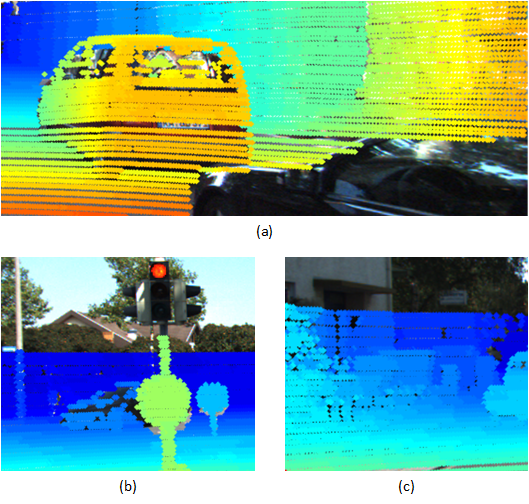
\includegraphics[width=0.7\textwidth]{visib_def_lidar.png}
%	\caption[LiDAR data projection]{Images with LiDAR data projection for examples in Figure \ref{figure:visib_def} (a), (b), and (c) respectively.}
%	\centering
%	\label{figure:visib_def_lidar}
%\end{figure}

\subsubsection{Possible Improvements}

KITTI offers the LiDAR data for all images, which can provide the depth information of each pixel point in the image or at least of a very small region. And based on the ground truth of location, orientation, and dimension of vehicles given by KITTI, we can calculate the depth of points distributed on the surface of the vehicles. By comparing these two kinds of depth information, we can correctly figure out whether there is some object in front of the target vehicle or not and which parts of the target vehicle are occluded, and thus we can classify the visibility properties correctly. Figure \ref{figure:visib_def} (d), (e) and (f). shows the images with LiDAR projection for (a), (b and (c). With the LiDAR depth information, we can easily classify the points around rear in (a) as self-occluded, and the occluded objects in (b) and (c) can be clearly detected and thus, we can assign the points whose depth is deeper than these objects as occluded. Therefore, for more accurate visibility labelling, it is worth making use of the LiDAR data.

\subsection{Deficiency of Template Matching}
In our approach, there are two situations where template matching is performed to fit a target vehicle with a 3D vehicle model. The first one is during labelling, when a 3D vehicle sketch is required to be projected into the KITTI images to generate 2D coordinates of key points of a target vehicle. And the model is selected via dimension matching. Another is during inference phase, where one 3D sketch is needed to generate the corresponding 3D coordinates of the key points for the target vehicle in the world coordinate system. This time the model is selected based on the estimated dimension proximity vector, \ie the ratios of 3 dimensions between the target vehicle and all 3D vehicle models.

In both cases, the most fundamental drawback is that we can only match the target vehicle with an approximate model based on the Dims strategy. This would result in errors in 2D and 3D coordinates of key points and thus impacts the final 3D vehicle pose estimation.

\subsubsection{Possible Improvements}
As we mentioned before, the geometric property of 3D sketch relies heavily on the type of the vehicles. Therefore, a possible improvement for matching is to introduce type information into the matching phase. And there are some out-off-shelf frameworks can provide this kind of information \cite{DBLP:journals/corr/YangLLT15, 7780697, 7410527, DBLP:journals/corr/DehghanMSO17}, \ie Afshin \etal provide a network which can recognize the Make and Model of vehicles \cite{DBLP:journals/corr/DehghanMSO17}. 

In sum, the optimal matching strategy is that we first collect a 3D vehicle dataset where the distribution of vehicle dimensions covers the main part of the distribution of real vehicle dimensions in a fine-grained style, and during the matching, we first estimate the type of the vehicle and then select the best model via dimension matching from the same category. 

\subsection{Deficiency of Input Image Format}

Now our network takes fixed-size patches as inputs which are generated by extracting, zero-padding, and resizing the 2D bounding box regions and then extracts features from these wrapped patches for regression and classification tasks. The data input mode is in spirit similar to R-CNN \cite{DBLP:journals/corr/GirshickDDM13}, where we have to process one KITTI image multiple times to estimate all vehicles in it. The reason why we use this data input format is to make sure that the input images in one mini-batch have the same size to fully utilize the efficient matrix multiplication, even if the 2D bounding box size is varying among different vehicles.

Even if no extra computation is wasted on the non-vehicle regions, the multiple-time input mode is not optimal because the patch generation stage is separated from the network and it is cumbersome to test different input formats, \ie patch scales and data augmentation.

\subsubsection{Possible Improvements}
In the future, we plan to exploit the Fast-RCNN \cite{DBLP:journals/corr/Girshick15} data input mode rather than R-CNN mode. The network first takes one entire KITTI image and its 2D bounding boxes as inputs, generates a shared feature map based on this image and then extracts a fixed-size feature vector from each feature map portion corresponding to its 2D bounding box one by one for later predictions. This functionality is realized mainly by introducing an ROI pooling layer described in \cite{DBLP:journals/corr/Girshick15}.

Not like Fast-RCNN \cite{DBLP:journals/corr/Girshick15}, the number of ROI, \ie bounding boxes, is dynamic for different images in our case. Therefore, we have to construct a dynamic computation graph for the network during training and inference. This is why we have not used this alternative up till now because we first implement the network in a static mode in Keras \cite{chollet2015keras} with TensorFlow \cite{tensorflow2015-whitepaper} as backend and it is hard to realize our functionality with them. Therefore, in the future, we will make use of libraries, \ie PyTorch \cite{paszke2017automatic}, to implement this alternative.

In this way, we can process the whole image one time rather than multiple times which can improve the process speed. What is more important is that we can easily modify how large the feature map portions are used to generate a fixed-size feature vector. Based on this, we can easily evaluate whether the additional context region around the 2D bounding boxes are beneficial for 3D pose estimation and if so, how much context information can boost the performance most.  


\subsection{Deficiency of the Whole Approach}
The first unpleasant thing about this approach is the additional labelling work. This is so time consuming that it takes more than two months to find a proper method to generate the additional labels at an acceptable accuracy level. Besides, even with this method, the accuracy of the labels is compromised.

Moreover, our approach requires an additional 3D vehicle model dataset to encode the geometry information of vehicles, which makes it hard to generalize to vehicles without a corresponding model in the model dataset. For example, our approach can't perform accurate 3D pose estimation of buses because we don't include the bus models.

According to the competition results of KITTI 3D object detection, the approach that relies on single sensor cannot compare with those making use of multi-sensor data \cite{3dobject}. RGB images captured by cameras have high resolution and good texture knowledge but lack depth information, while cloud points collected by LiDAR have 3D information of the scene but the resolution is relatively lower and lack texture information. Therefore, we think the best performance would be achieved by some approach driven by sensor fusion. If we can start this task again, this is the first direction we will explore.


\clearpage

\section{Conclusion}
 This thesis deals with the problem of 3D pose estimation of vehicles based on monocular images by using deep neural networks for the application of autonomous driving. We train a deep neural network to predict 2D coordinates and visibility property for characteristic points, as well as a dimension proximity vector, for a target vehicle. During the inference phase, we first perform template matching to reason out the target vehicle's 3D dimensions and 3D coordinates of the key points with the help of the dimension proximity vector and 3D vehicle dataset, and finally, 2D-3D matching is performed to recover the location and orientation of the vehicle. Combining the network and inference phases, our approach can simultaneously perform 3D bounding box estimation, 3D localization, 3D orientation estimation, 3D dimension estimation, 2D part localization, and parts visibility characterization for a vehicle in a 2D bounding box patch. 
 
Our work achieves state-of-the-art performance on six tasks. It outperforms most monocular methods recorded in KITTI 3D object detection competition on the most important task, 3D vehicle detection. Besides, our network can predict 2D coordinates and dimension proximity vector for highly occluded or truncated vehicles and therefore, our approach can perform template matching and 2D-3D matching to recover their 3D bounding boxes. Moreover, unlike other methods, our approach can provide more detailed information of the detected vehicle, \eg 2D part location and 2D part visibility, which is useful for autonomous driving applications to gain a more  fine-grained perception. Finally, the runtime for our approach is at real time level, \textit{ca.} 0.02s per image on one GeForce GTX TITAN X GPU. 

In order to maximize the effective capacity of the model, we thoroughly research and evaluate the key design alternatives and hyperparameters, including loss function, loss weight, learning rate, weight decay, base net feature extractor, model selection strategy, and the number of points used in a model. Based on these experiments, the performance of our approach is boosted steadily and finally reaches the state-of-the-art level.

Finally, we present results of these six tasks and compare them with other methods. We also describe the deficiencies of our approach, analyse their causes, and propose possible solutions which are the directions for future improvements. 
\clearpage

\bibliographystyle{unsrt}
\bibliography{reference}
\clearpage
%\printbibliography


%\begin{appendices}
%	\section{List of Figures and Tables}
%	\listoffigures
%	\clearpage
%	\listoftables
%	\clearpage
%\end{appendices}

\section*{Acknowledgement}
I really appreciate the wholehearted support from my family throughout my endless and challenging  study, especially for this oversea period. Special thanks belong to my supervisors, Hung Ngo at MLR and Jie Zhong at Bosch, for giving me this opportunity to work on this challenging and interesting topic. And I would like to thank them for their guidance and help during the past six months. And I am also grateful to my friends, Ze Guo, Haonan Zhang and Yujin Wang for their inspirations and help. Moreover, I harbour sincere gratitude for the Yi's company in the last ten days when I was struggling with revising. Finally, I am thankful to my friends for their forgiveness for and consideration of my absence in the final month.

\Affirmation
\end{document}